%%%%%%%%%%%%%%%%%%%%%%
%%%%%% PACKAGES %%%%%%
%%%%%%%%%%%%%%%%%%%%%%

%%%%%%%%%%%%%%%%%
%%% Mandatory %%%
%%%%%%%%%%%%%%%%%
\documentclass[11pt,twoside,a4paper]{report}
\usepackage[DETI,newLogo]{uaThesis}
\usepackage{float}

%%%%%%%%%%%%%%%%
%%% Optional %%%
%%%%%%%%%%%%%%%%
\usepackage[english]{babel}
\usepackage{hyperref}
\usepackage{amsmath}
\usepackage{amssymb}
\usepackage{xspace}% used by \sigla
\usepackage{lipsum}
\usepackage[T1]{fontenc}
\usepackage[backend=biber, refsegment=chapter, sorting=none, url=false, doi=false]{biblatex}

\bibliography{thesisBib.bib}  %% bibliografia

\usepackage{csquotes}
\usepackage[acronym,nonumberlist]{glossaries}
\newglossary[tlg]{nomenclature}{tld}{tdn}{Nomenclature}
\usepackage{xcolor}
\setlength {\marginparwidth }{2cm}
\usepackage{todonotes}
\usepackage[bottom]{footmisc}
\usepackage{amsmath}
\usepackage{xfrac}
\usepackage{tikz}
\usepackage{mathdots}
\usepackage{yhmath}
\usepackage{cancel}
\usepackage{color}
\usepackage{siunitx}
\usepackage{array}
\usepackage{multirow}
\usepackage{amssymb}
\usepackage{gensymb}
\usepackage{tabularx}
\usepackage{booktabs}
\usetikzlibrary{fadings,shapes,arrows,chains,backgrounds,calc,arrows,arrows.meta,shadows,shapes.geometric, fit, positioning}
\usepackage{caption,subcaption}
\usepackage{epstopdf}
\usepackage{mathtools, nccmath}
\usepackage{pdflscape}
\usepackage{afterpage}
\usepackage{url}
\PassOptionsToPackage{hyphens}{url}
\usepackage{nomencl}
\makenomenclature   

%%%%%%%%%%%%%%%%%%%%%%%
% Tikz library and set
\usepackage{tikz}

\usetikzlibrary{arrows}
\usetikzlibrary{positioning} 
\usetikzlibrary{matrix}

\tikzset{
    %Define standard arrow tip
    >=stealth',
    %Define style for boxes
    process/.style=  {
                     rectangle,
                     draw=black, very thick,
                     text width=6.5em,
                     minimum height=2em,
                     text centered
                     },
    secProc/.style=  {
                     rectangle,           
                     rounded edge,
                     draw=black, very thick,
                     minimum height=2em,
                     text centered
                     },
    % Define arrow style
    pil/.style={
           ->,
           thick,
           shorten <=2pt,
           shorten >=2pt,}
}

\def\checkmark{\tikz\fill[scale=0.4](0,.35) -- (.25,0) -- (1,.7) -- (.25,.15) -- cycle;} 

%%%%%%%%%%%%%%%%%%%%%%%
%%%% Header makeup %%%%
%%%%%%%%%%%%%%%%%%%%%%%

%\usepackage[Sonny]{fncychap}
%\ChNameVar{\Huge\bfseries}
%\ChNumVar{\Huge\bfseries}
%\ChTitleVar{\LARGE\bfseries}
\usepackage{color}
\definecolor{gray75}{gray}{0.75}
\usepackage{titlesec}

\titlespacing*{\chapter}{0pt}{-10pt}{60pt}

\titleformat{\chapter}[display] % shape
{\bfseries\LARGE} % format
{\MakeUppercase{\chaptertitlename} \Huge\thechapter} % label
{0.5ex} % sep
{\titlerule\vspace{1ex}\filleft}
[\vspace{1ex}\titlerule]

\newcommand{\dgrayvline}{\raisebox{-0.5ex}{\tikz\filldraw[darkgray,x=2pt,y=2pt] (0,0) -- ++(0.5,0) -- ++(0,1em) -- ++(-0.5,0) -- cycle;}}

\titleformat{\section}[hang]
{\Large\bfseries}
{\thesection\hspace{25pt}\dgrayvline\hspace{10pt}}
{0pt}
{\Large\bfseries}

\newcommand{\grayvline}{\raisebox{-0.5ex}{\tikz\filldraw[gray,x=2pt,y=2pt] (0,0) -- ++(0.5,0) -- ++(0,1em) -- ++(-0.5,0) -- cycle;}}

\titleformat{\subsection}[hang]
{\large\bfseries}
{\thesubsection\hspace{18pt}\grayvline\hspace{10pt}}
{0pt}
{\large\bfseries}

\newcommand{\lgrayvline}{\raisebox{-0.5ex}{\tikz\filldraw[lightgray,x=2pt,y=2pt] (0,0) -- ++(0.5,0) -- ++(0,1em) -- ++(-0.5,0) -- cycle;}}

\titleformat{\subsubsection}[hang]
{\normalsize\bfseries}
{\thesubsubsection\hspace{10pt}\lgrayvline\hspace{10pt}}
{0pt}
{\normalsize\bfseries}

\newcommand{\textsep}{\noindent\makebox[\linewidth]{\resizebox{0.3333\linewidth}{1pt}{$\bullet$}}\bigskip}


%%%%%%%%%%%%%%%%%%%%%%
%%%%%%% MACROS %%%%%%%
%%%%%%%%%%%%%%%%%%%%%%

%%%%%%%%%%%%
% TOS
\setcounter{tocdepth}{2}
\setcounter{secnumdepth}{3}
% optional (comment to used default)
%   horizontal line to separate floats (figures and tables) from text
%\def\topfigrule{\kern 7.8pt \hrule width\textwidth\kern -8.2pt\relax}
%\def\dblfigrule{\kern 7.8pt \hrule width\textwidth\kern -8.2pt\relax}
%\def\botfigrule{\kern -7.8pt \hrule width\textwidth\kern 8.2pt\relax}

% custom macros (could also be defined using \newcommand)
\def\I{\mathtt{i}}         % one possible way to represent $\sqrt{-1}$
\def\Exp#1{e^{2\pi\I #1}}  % argument inside braces, i.e., "{}"
\def\EXP#1.{e^{2\pi\I #1}} % argument finishes when a full stop is encountered, i.e., "."
\def\sigla{\LaTeX\xspace}  % use as "blabla \sigla blabla (no need to do "blabla \sigla\ blabla"

\def\AddVMargin#1{\setbox0=\hbox{#1}%
                  \dimen0=\ht0\advance\dimen0 by 2pt\ht0=\dimen0%
                  \dimen0=\dp0\advance\dimen0 by 2pt\dp0=\dimen0%
                  \box0}   % add extra vertical space above and below the argument (#1)
\def\Header#1#2{\setbox1=\hbox{#1}\setbox2=\hbox{#2}%
           \ifdim\wd1>\wd2\dimen0=\wd1\else\dimen0=\wd2\fi%
           \AddVMargin{\parbox{\dimen0}{\centering #1\\#2}}} % put #1 on top #2

%%%%%%%%%%%%
% Mine
\def\ThesisYear{\the\year}
\def\myName{Júlio Miguel Braz da Costa Silva}
\def\TituloTese{Recuperação e Identificação de Momentos em Imagens/Vídeos}
\def\ThesisTitle{Recovery and Identification of Moments in Images / Videos}

\setlength\bibitemsep{2.5\itemsep}        % Aumenta espaçamento entre entradas da bibliografia

\emergencystretch=20em                     % Corrigir overfull hbox

\setlength{\parskip}{0ex}

\newcommand{\figwidth}{0.6\textwidth}

\renewcommand{\arraystretch}{1.2}
\setlength{\tabcolsep}{12pt}

\DeclarePairedDelimiter{\nint}\lfloor\rceil
\DeclarePairedDelimiter{\nfloor}\lfloor\rfloor
\DeclarePairedDelimiter{\nceil}\lceil\rceil

\interfootnotelinepenalty=10000         % Change priority for footnotes

\newcommand{\todor}[1]{\todo[inline, color=red!40]{#1}}
\newcommand{\pathcos}[6]{\path (#1.east) to node [pathcos, color=#5, #6] {$\sfrac{#3\pi}{#4}$} (#2.west)}

%%%%%%%%%%%%%%%%%%%%
% Carregar Glossário
\makenoidxglossaries
\loadglsentries{glossary}

%%%%%%%%%%%%%%%%%%%%%%%%%%%%%%%%%%%
%%%%%%%%% BEGIN DOCUMENT %%%%%%%%%%
%%%%%%%%%%%%%%%%%%%%%%%%%%%%%%%%%%%
\begin{document}

%%%%%%%%%%%%%%%%%%%%%%%%%%%%%%%%%%%%%%%%%%%%%%%%%%%%%%%%%%%%%%%%
% Capa, contracapa, Júri, agradecimentos, palavras chave, resumo
% CoverPage
\TitlePage

  \HEADER{\BAR}
         {\ThesisYear}
  \TITLE{\myName}
        {\TituloTese}
        {\ThesisTitle}
\EndTitlePage
\titlepage\ \endtitlepage % empty page


%
% Initial thesis pages
%

\TitlePage
  \HEADER{}{\ThesisYear}
  \TITLE{\myName}
        {\TituloTese}
        {\ThesisTitle}
  \vskip 15mm
  \TEXT{}
       {Dissertação de Mestrado apresentada à Universidade de Aveiro, para obtenção do grau de Mestre em Engenharia Eletrónica e de Telecomunicações, sob orientação cientifica Professor Doutor António Neves, Professor do Departamento de Eletrónica, Telecomunicações e Informática da Universidade de Aveiro e coorientação de Ricardo Ribeiro, Investigador no Instituto de Engenharia Eletrónica e Telemática de Aveiro da Universidade de Aveiro.}
\EndTitlePage
\titlepage\ \endtitlepage % empty page

\TitlePage
  \vspace*{55mm}
  \TEXT{\textbf{o júuri~/~the jury\newline}}
       {}
  \TEXT{presidente~/~president}
       {\textbf{ABC}\newline {\small
        Professor Catedr\'atico da Universidade de Aveiro (por delega\c c\~ao da Reitora da
        Universidade de Aveiro)}}
  \vspace*{5mm}
  \TEXT{vogais~/~examiners committee}
       {\textbf{DEF}\newline {\small
        Professor Catedr\'atico da Universidade de Aveiro (orientador)}}
  \vspace*{5mm}
  \TEXT{}
       {\textbf{GHI}\newline {\small
        Professor associado da Universidade J (co-orientador)}}
  \vspace*{5mm}
  \TEXT{}
       {\textbf{KLM}\newline {\small
        Professor Catedr\'atico da Universidade N}}
\EndTitlePage
\titlepage\ \endtitlepage % empty page

\TitlePage
  \vspace*{55mm}
  \TEXT{\textbf{agradecimentos~/\newline acknowledgements}}
       {Aos meus pais e à minha irmã por ao longo dos anos terem sido sempre imprescindíveis, nunca me terem faltado, proporcionando sempre todo o apoio necessário e condições que me levaram a alcançar os meus objetivos e me tornar a pessoa que hoje sou.}
  
  \TEXT{}
       {Aos meus amigos de Tondela que tanta paciência tiveram para me aturar ao longo dos anos.}
       \TEXT{}
       {Aos amigos que Aveiro me proporcionou que tantas histórias criámos juntos.}

       \TEXT{}
       {À Mariana Coutinho por todos os bons momentos, apoio, carinho e companheirismo que me facilitaram este último ano.}

       \TEXT{}
       {Ao meu colega de casa Pedro Nunes a pessoa com quem tantas longas conversas tive e a que mais me chateou a cabeça para despachar as cadeiras e a dissertação. 
       }
       \TEXT{}
       {Ao professor António Neves que apesar das dificuldades impostas pelo trabalho à distância sempre me motivou e orientou, sugerindo sempre possíveis soluções e caminhos a percorrer. }
       \TEXT{}
       {Ao Ricardo Ribeiro que tanta disponibilidade teve para me ajudar com todas as minhas dúvidas. Uma ajuda fundamental no trabalho realizado.}
\EndTitlePage
\titlepage\ \endtitlepage % empty page

\TitlePage
  \vspace*{55mm}
  \TEXT{\textbf{Palavras-Chave}}
       {\textbf{Visão por Computador, Processamento Natural de Texto, ImageClef, Lifelogging, Recuperação de Momentos}}

          
     \TEXT{\textbf{Resumo}}
      {Na sociedade moderna, praticamente qualquer pessoa consegue capturar momentos e registar eventos devido à facilidade de acesso a \textit{smartphones}. Isso leva à questão, se registamos tanto da nossa vida, como podemos facilmente recuperar momentos específicos? A resposta a esta questão abriria a porta para um grande salto na qualidade da vida humana. As possibilidades são infinitas, desde problemas triviais como encontrar a foto de um bolo de aniversário até ser capaz de analisar o progresso de doenças mentais em pacientes ou mesmo rastrear pessoas com doenças infecciosas.}

     \TEXT{}
     {Com tantos dados a serem criados todos os dias, a resposta a esta pergunta torna-se mais complexa. Não existe uma abordagem linear para resolver o problema da localização de momentos num grande conjunto de imagens e investigações sobre este problema começaram há apenas poucos anos. O ImageClef é uma competição onde investigadores participam e tentam alcançar novos e melhores resultados na tarefa de recuperação de momentos a cada ano.}

     \TEXT{}
     {Este problema complexo, em conjunto com o interesse em participar na tarefa LMRT do ImageClef, apresentam-se como um bom desafio para o desenvolvimento desta dissertação.}

     \TEXT{}
     {A solução proposta consiste num sistema capaz de recuperar automaticamente imagens de momentos descritos em formato de texto, sem qualquer tipo de interação de um utilizador, utilizando apenas métodos estado da arte de processamento de imagem e texto.} 

     \TEXT{}
     {O sistema de recuperação desenvolvido alcança este objetivo através da extração e categorização de informação relevante de texto enquanto calcula um valor de similaridade com os rótulos extraídos durante a fase de processamento de imagem. Dessa forma, o sistema consegue dizer se as imagens estão relacionadas ao momento especificado no texto e, portanto, é capaz de recuperar as imagens de acordo.
     }

     \TEXT{}
     {Na subtarefa ImageCLEF Life Moment Retrieval 2020, o sistema de recuperação automática de imagens proposto alcançou uma pontuação de 0,03 na metodologia de avaliação F1-measure@10. Mesmo que estas pontuações não sejam competitivas quando comparadas às pontuações de outros sistemas de outras equipas, o sistema construído apresenta-se como uma boa base para trabalhos futuros.}


\EndTitlePage
\titlepage\ \endtitlepage % empty page

\TitlePage
  \vspace*{55mm}
  \TEXT{\textbf{Keywords}}
       {\textbf{Computer Vision, Natural Language Processing, ImageCleff, Lifelogging, Moment Retrieval}}

     \TEXT{\textbf{Abstract}}
     {In our modern society almost anyone is able to capture moments and record events due to the ease accessibility to smartphones. This leads to the question, if we record so much of our life how can we easily retrieve specific moments? The answer to this question would open the door for a big leap in human life quality. The possibilities are endless, from trivial problems like finding a photo of a birthday cake to being capable of analyzing the progress of mental illnesses in patients or even tracking people with infectious diseases.}

     \TEXT{}
     {With so much data being created everyday, answering the question becomes complex. There is no stream lined approach to solve the problem of moment localization in a large dataset of images of and investigation into this problem have only started a few years ago. ImageClef is one competition where researchers participate and try to achieve new and better results in the task of moment retrieval.}

     \TEXT{}
     {This complex problem, along with the interest in participating in the ImageClef Life Moment Retrieval Task posed a good challenge for the development of this dissertation.}

     \TEXT{}
     {The proposed solution consists in developing a system capable of retriving images automatically  according to specified moments described in a corpous of text without any sort of user interaction using only state-of-the-art image and text processing methods.}

     \TEXT{}
     {The developed retrieval system achieves this objective by extracting and categorizing relevant information from text while being able to compute a similarity score with the extracted labels from the image processing stage. In this way, the system is capable of telling if images are related to the specified moment in text and therefore able to retrieve the pictures accordingly.}

     \TEXT{}
     {In the ImageCLEF Life Moment Retrieval 2020 subtask the proposed automatic retrieval system achieved a score of 0.03 in the F1-measure@10 evaluation methodology. Even though this scores are not competitve when compared to other teams systems scores, the built system presents a good baseline for future work. }

\EndTitlePage
\titlepage\ \endtitlepage % empty page



%%%%%%%%%%%%%%%%%%%%%%%%%%%%%%%%%%%%%
% Tables of contents, of figures, ...
\pagenumbering{roman}
\tableofcontents

\cleardoublepage
\listoffigures
\addcontentsline{toc}{chapter}{\listfigurename}

\cleardoublepage
\listoftables
\addcontentsline{toc}{chapter}{\listtablename}

\cleardoublepage
\printnoidxglossary[type=\acronymtype]
\addcontentsline{toc}{chapter}{\acronymname}

\cleardoublepage
\printnoidxglossary
\addcontentsline{toc}{chapter}{\glossaryname}


%%%%%%%%%% Descomentar para adicionar nomenclatura
\cleardoublepage
\printnoidxglossary[type=nomenclature,title=Nomenclature]
\addcontentsline{toc}{chapter}{Nomenclature}


%%%%%%%%%%%%%%%%%%%%%%%%%%%%%%%%%%%%%
\pagenumbering{arabic}
% Introduction

\cleardoublepage

\chapter{Introduction}
\label{ch:introduction}
This chapter gives an introduction to the surrounding theme addressed in this thesis. In that sense, firstly the contextualization of the theme and the respective motivation will be presented. The different challenges, the objectives that are intended to be reach and the contributions given to the community are also described. Finally the document structure and organization is explained.


\section{Context and Motivation}

The pervasive creation and consumption of visual media content is ingrained into our modern world. In the past, the main purpose given to pictures was to save moments of events. Nowadays people are constantly consuming visual media content. Pictures, images and photos have many different usages, not only we use them for social media but also we use them in engineering, in art, in science, in medicine, in entertainment and also in advertising \cite{Zhang2008}.



With the rapid development of Internet of things (IOT) this growth in consumption of visual media content has increased the usage of wearable and smart technologies making the subject of lifelogging more prevalent in the recent years. Lifelogging is the task of tracking and recording personal data created trough the activities and behaviour of individuals during their day-to-day life in the form of images, video, biometric data, location and other data. The name given to the data created by lifelogging has the name of "lifelog data" and it is rich in resources for contextual information retrieval \cite{Ribeiro}.

Some great examples of the usefulness of lifelogging is using it as memory extension for people who suffer from memory impairments such as Alzheimers, to find lost items during the day or even to understand human behaviour.

The problems related to creating, compressing, storing, transmitting, rendering and protecting image data are already solved. However there still exists two difficult problems to tackle which are the issues associated with image location and the continuous growth of image data (big data) \cite{Zhang2008}.

"Locating images involves analysing them to determine their content, classifying them into related groupings, and searching for  images. In order to solve these problems, the current technology relies heavily on the image description" \cite{Zhang2008}, usually called as "image metadata". This data can either be added automatically at the capturing time or manually added by someone afterwards.

According to the literature \cite{Zhang2008} : "In the present time the development in the area of content–based analysis (indexing and searching of visual media) is increasing, this is where most of the research in image management is concentrated. Automatic analysis of the content of images, which in turn would open the door to content–based indexing, classification and retrieval, is an inherently difficult problem and therefore progress is slow." 

However, if one day a fully automatic image/video retrieval system is implemented it will vastly improve the life quality of the human kind. A great example that we can apply at the present time is that it will be possible to backtrack the last few days of humans infected with COVID-19 through their lifelog data, which in turn would help to identify more possible infected and warn more people to get tested.

\section{Challenges}

As it has been described earlier in the chapter, creating an automatic system capable of fully analysing the content of images is a difficult problem. This difficulty comes from two main challenges which are image processing and text processing. 

Creating an automatic system capable of image retrieval means that the computer has to be able to understand images and text while at the same time being capable of relating both.

For the image processing challenge, the computer has to be able to extract relevant information from images like colors, objects, places, locations, indoor or outdoors, activities happening in the photo, people, etc. However in order to do this,  many different algorithms have to be implemented like object detection, activity recognition, scene recognition and others. The usage of so many algorithms can require extreme computational time and resources depending on the size of the dataset to be analysed. If one image requires 1 second to be fully processed, a dataset of 200.000 images of the same resolution would require approximately 2 days.

In order to teach the computer to understand text there has to be an underlying understanding of the language. Natural Language Processing algorithms have to be implemented, however these algorithms only allow the computer to extract the basics like which words are verbs, adjectives, nouns, etc. With this in mind, another algorithm has to be fully written from scratch capable of using that data to extract activities, locations, people, dates, indoor or outdoor, etc from a corpus of text.

Finally, the computer has to be capable of comparing the extracted features from the text with extracted features from the images, in order to associate images to text.

\section{Objectives}

The main objective of this work is to develop an automatic image retrieval system capable of participating in the ImageCLEF LMRT-subtask challenge (described in chapter \ref{ch:imageclef}). In order to achieve this the following bullet points have to be accomplished :

\begin{itemize}
    \item Study on the state of the art of image processing and text processing algorithms.
    \item Choice of the main algorithms to be used.
    \item Choice of the Python libraries to be used.
    \item Code of an algorithm capable of processing images and extract relevant features.
    \item Code of an algorithm capable of processing text and extract relevant features.
    \item Code of an algorithm able to compare the extracted features from the images with the extracted features from the text and capable of associating images to text.
    \item Code of an algorithm capable of calculating the F1@score of the final results.
    \item Code of a batch script in order to make the system run with one click.
  \end{itemize}


\section{Contributions}

Since the process of automatic image retrieval is still complex problem this works aims at contributing with a baseline system for future investigations with some suggestions on how to improve it further. Additionally a deep study of the available technology is realized that may help on finding new paths for automatic image retrieval.


\section{Document Structure}
This document has a total of XX chapters that are divided accordingly:




\begin{itemize}
  \item Chapter \ref{ch:introduction}: Presents the context and motivation along with the challenges and objectives.
  \item Chapter \ref{ch:computervision}: Provides a survey on the subject of feature extraction from images and video.
  \item Chapter \ref{ch:nlp}: Addresses the thematic of natural language processing.
  \item Chapter \ref{ch:imageclef}: Discusses the imageCLEF challenge.
  \item Chapter \ref{ch:initial_work}: Provides an overview of the system created and the steps that took to achieve its final state.
  \item Chapter \ref{ch:conclusion}: Describes the conclusions taken from the development of the work and provides some ideas for future work and investigations.
  
 
 
\end{itemize}



\cleardoublepage

\chapter{imageClef}
\label{ch:imageclef}

\cleardoublepage


\chapter{Information Extraction From Images}
\label{ch:computervision}



The task of automatically recognizing and locating objects in images and videos is of extreme importance for computers to be able to understand and interact with their surroundings. Some major applications of this particular task of object detection are pedestrian detection, surveillance, autonomous driving, text digitalization, face detection and recognition, robotics, object counting and so on \cite{Agarwal2019}. 

For this work the purpose of using object detection technologies is to convert images into text in order to allow the computer to compare an image with a moment described in text.

Feature extraction plays an important role in image classification and object detection systems which are two core components of computer vision. To put in simple terms, feature extraction is the first step in converting an image into text \cite{Tiwari2013}. Figure \ref{fig:feature_extraction} shows an example of feature extraction. However, the computer is only capable of learning that the extracted features represent a motorcycle after classifying the extracted data, which is done with the usage of pre-trained deep learning neural networks.





\begin{figure}[H]
    \centering
    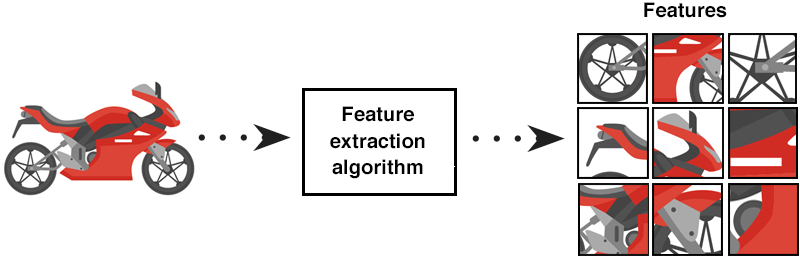
\includegraphics[scale = 0.55]{Sections/2StateOfTheArt/2_images/Feature_extraction.png}
    \caption{Feature extraction from an image. \cite{feature} }  
    \label{fig:feature_extraction}
\end{figure}


\par This chapter starts with fundamental concepts in Section \ref{sec:fundamental}. Section \ref{sec:libraries_cv} gives a brief introduction of the most common computer vision libraries. Neural networks are introduced in Section \ref{sec:neuralnet}, where the most common architecture types are presented. Finally, a state-of-the-art in object detection and image classification can be read in Section \ref{sec:state}.

\newpage

    
\section{Concepts of Label Extraction}
\label{sec:fundamental}



%%%%%%%%%%%%%%%%%%%%%%%%%%%%%%%%%%%%%%%%%%%%%%%%%%%%%%%%%%%%%%%%%%%%%%%%%%%%%

\begin{itemize}
    \item \textbf{Features and Feature Space}
\end{itemize}

    \label{sec:featurespace}
    \par A feature is considered to be a measurable piece of data in the image which is unique to a specific object, it can be color, texture or shape. Usually this features are extracted from the image and used in order to represent an object. Color is the most straightforward visual feature for indexing and image retrieval, while shape representation is the most difficult. This is because a 3-D real world object is represented in a 2-D plane in an image, which means that one dimension of information is completely lost. Texture features are very important in pattern recognition and is an important cue in region based segmentation of images.

    \par The similarity between images can be determined through features which are represented as a vector. 

    \par To sum things up, feature space is a collection of features related to some properties of the object, while a feature is an individual measurable characteristics of the object \cite{Tiwari2013}.

    %%%%%%%%%%%%%%%%%%%%%%%%%%%%%%%%%%%%%%%%%%%%%%%%%%%%%%%%%%%%%%%%%%%%%%%%%%%%%
    \begin{itemize}
        \item \textbf{Objects}
    \end{itemize}

 
    \par An object is used to identify specific items in an image or specific frames in a video. It is possible to label multiple objects in an image. An example of objects in an image of a car might be wheels, headlights, etc.
    \par Usually an object is represented by a group of features in form of a feature vector that is used to recognize objects and classify them \cite{Tiwari2013}.

    \par In object detection, small objects are normally the ones that give  worst results and lower performance when being detected. This happens because the information available to detect them is more compressed and hard to decode without some prior knowledge or context \cite{Agarwal2019}.

%%%%%%%%%%%%%%%%%%%%%%%%%%%%%%%%%%%%%%%%%%%%%%%%%%%%%%%%%%%%%%%%%%%%%%%%%%%%%%

\begin{itemize}
    \item \textbf{Image Annotation and Classification}
\end{itemize}

    Image classification is the process of associating an entire image with just one label. A simple example of image classification is labeling types of animals, cars or plants \cite{Feng2019}. \par
    Image annotation, one of the most important tasks in computer vision, is the process of annotating an image with labels. These labels are predetermined in order to give the computer vision model information about what is shown in the image, they are a combination of a bounding box in specific coordinates of the image  and a description of the object inside of it \cite{annotation}. \par

    Feeding this kind of annotated image data to a computer model teaches it to recognize the visual characteristics of that specific label, this makes the model able to categorize new unannotated images of the same type of that label. Some of these models are presented in Appendix \ref{ch:appendix}.

    \begin{itemize}
        \item \textbf{Object Detection, Segmentation and Recognition}
    \end{itemize}
    

    \par Object detection is the name given to the process that combines image classification with object localization \cite{ObjectDetection}. As previously explained, image classification is the prediction and assignment of a class label to an image, while object localization is the prediction and drawing of a bounding box around one or more objects in the image. In other words, object detection is the task that deals with the detection of objects of a certain class (e.g "flower","table","plane") in images, making it a natural extension of the classification problem. 

    \par The object detection task is considered to be a supervised learning problem, since the objective is to design an algorithm which can accurately locate and correctly classify as many instances of objects as possible, in a bounding box, while avoiding false detections in a given set of training images.  As an added challenge, many object detection applications require the problem to be solved in real time, which can be achieved. However, in order for a detector to be faster, accuracy is usually reduced. 

    \par Finally, object segmentation is the task of grouping pixels from the same object into a single region and object recognition is usually defined as giving the name of the category of an object that is contained in an image or a bounding box, assuming there is only one object in the image. For some authors object recognition can also involve detecting all objects in an image \cite{Agarwal2019}.

    A survery on classification and regression based algorithms for object detection can be read in Appendix \ref{ch:appendix}.

 

    \begin{itemize}
        \item \textbf{Image Description}
    \end{itemize}


    \par Image description is the meaning of an image and humans can understand it with relative ease. However computers only see the digital representation of images, only detecting pixels, and therefore they are not able to recognize the semantic of the image. This problem makes the semantic gap the main challenge in computer vision \cite{Huang2012}. This gap is defined by the lack of coincidence between the information extracted from visual data and the interpretation in a given situation \cite{Agarwal2019}.
    


    \par As an example, picture \ref{fig:picnic} shows an image of a family having a picnic. Feeding this image to a computer will output very different results from what a human would say.

    \begin{figure}[H]
        \centering
        \captionsetup{justification=centering}
        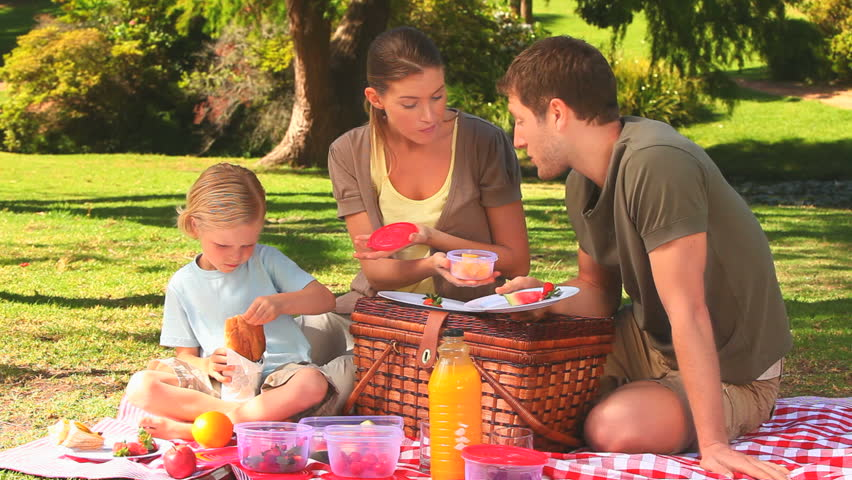
\includegraphics[width=0.5\textwidth]{Sections/2StateOfTheArt/2_images/picinic.png}
        \caption{Generic picture of a family having a picnic.}
        \label{fig:picnic}  
    \end{figure}

    Using google cloud vision API \cite{google} to extract information from the image, the following data is what the computer outputs:

    \begin{itemize}
        \item \textbf{Objects}: Person - 89\%, Person - 86\%, Person - 82\%, Tableware -59\%, Tableware - 55\%, Package goods - 54\%, Package goods - 50\%. 
        \item \textbf{Labels}: Picnic - 93\%, Recreation - 86\%, Sharing - 82\%, Event - 74\%, Summer - 70\%, Child - 61\%, Play - 57\%, Family - 52\%, Lunch - 52\%.
    \end{itemize}
   
   However, the human output would be: 
   
   \begin{itemize}
       \item \textbf{Sentence}: A family having a picnic in the park.
   \end{itemize}

     
    \par A computer is only capable of outputting the objects and labels detected but is incapable of giving them any sort of meaning like a human can.



%%%%%%%%%%%%%%%%%%%%%%%%%%%%%%%%%%%%%%%%%%%%%%%%%%%%%%%%%%%%%%%%%%%%%%%%%%%%%%


%%%%%%%%%%%%%%%%%%%%%%%%%%%%%%%%%%%%%%%%%%%%%%%%%%%%%%%%%%%%%%%%%%%%%%%%%%%%%%
    \section{Teaching a Computer on How to Learn}

    \begin{itemize}
        \item \textbf{ Artificial Intelligence }
    \end{itemize}

    Artificial Intelligence (AI) is the artificial simulation of human intelligence by a computer system in a way that it can perceive its environment, understand its behaviors and take action. Two important areas of AI are machine learning and deep learning \cite{mathworks_AI}.

    


    \begin{itemize}
        \item \textbf{Machine Learning}
    \end{itemize}
    

    \par Machine learning can be defined as a data analytics technique that allows computers to learn from experience. There are two types of machine learning techniques, which are supervised learning and unsupervised learning.
    \par Normally, supervised machine learning is used to train a model to predict future outputs, this is done by inputting and outputting known data. Supervised learning uses two different techniques which are classification and regression. Classification techniques are used to classify input data into categories while regression techniques are used to predict continuous responses. 
    \par Unsupervised learning is mostly used to find hidden patterns or intrinsic structures in input data. The most common unsupervised learning technique is clustering which is used for data analysis exploration, in order to find hidden patterns or groupings in data \cite{mathworks_ML}.

    \begin{itemize}
        \item \textbf{Deep Learning}
    \end{itemize}
    

    \par Deep Learning is a subset of Machine Learning that is inspired by the structure and function of the human brain. In order to achieve this, deep learning resorts to artificial neural networks (ANNs).
    
    \par The idea behind an ANN is that it tries to replicate the working of the human brain in the processing of data and creation of patterns, which is important for decision making. These ANNs are capable of learning unsupervised data that can either be unstructured, unlabeled or both. Putting it as simple as possible, deep learning is a machine learning technique that teaches computers to learn by example, like a human would \cite{mathworks_deeplearning}.


    \par Thanks to the new digital era, there has been an exponential increase in all forms of data, from every region of the planet. This data is defined as "big data" and comes from sources like social media, search engines, live streaming services and many others. Even though all of this information is easily accessible, it is unstructured. The problem with unstructured data is that the human brain cannot comprehend it efficiently enough to extract relevant information. However, using deep learning, all of this unstructured data can be usable.

    \par A computer model learns how to perform classification tasks directly from data, being it text, images or sound. Current deep learning models are able to achieve such levels of accuracy that they can outperform humans.

    \par In deep learning, models are trained with the usage of a large set of labeled data and neural network architectures that contain many layers. This is one of the disadvantages of deep learning, in order to improve the results of an ANN it requires to be trained with large amounts of labeled data. Since deep learning deals with such great volumes of information, this introduces another disadvantage to deep learning, which is the extreme need of higher and higher computing power.

   
        
    \par The term "deep" comes from the usage of an extensive quantity of hidden layers in the neural network. A normal neural network usually contains 2-3 hidden layers where as a deep neural network can go up to 150 hidden layers or more.

    \par As explained previously, deep learning models are trained by the usage of  large sets of labeled data and neural network architectures that are capable of automatically extracting features from the data, without the need for manual feature extraction. This automated feature extraction makes deep learning models highly accurate and practical for computer vision tasks such as object classification. 
    
    \par Deep Learning also offers "end-to-end learning", this means that a network can learn how to automatically classify raw data. In addition, deep learning algorithms scale with data, where as machine learning methods bottleneck at a certain level of performance when more examples and training data are added, which gives deep learning networks a key advantage since they improve as the size of the data increases \cite{mathworks_deeplearning}.


    The main purpose of deep learning, for this work, will be to apply it to the images provided by the imageCLEF challenge.
    
    \begin{itemize}
        \item \textbf{Computer Vision}
    \end{itemize}
    \par Computer vision is a field of artificial intelligence and computer science that aims at giving computers a visual understanding of the world \cite{cv} \cite{cv2}. It is related with pattern recognition, which is a common way to train a computer so that it can understand visual information. Pattern Recognition is the training a computer goes through when it is fed with different labeled images and then subjected to different algorithms, allowing the computer to hunt for patterns in every element related to those specific labels \cite{pattern}.


\subsection{Neural Networks}
\label{sec:neuralnet}

    \par A neural network can be considered a computer program that operates identically to how a human brain would, in the sense that it is able to be teachable to do certain tasks like problem-solving. The appeal of a neural network is the ability to emulate the human brain in pattern recognition skills. 


    \par Neural networks are composed of many small cells called neurons. These neurons are grouped into several layers that form columns. The connection between columns are formed also through their neurons. Each neuron of each layer is connected to another neuron of another layer. A visual representation of a generic neural network architecture is shown in figure \ref{fig:neural}. For further readings on neural network architectures Appendix \ref{ch:appendix} describes most of the common architectures.


    \begin{figure}[htb]
        \centering
        \includegraphics[scale = 0.5]{Sections/2StateOfTheArt/2_images/deeplearning.pdf}
        \caption{Typical neural network architecture \cite{mathworks_NN}.}
        \label{fig:neural}
    \end{figure}
        
    
    \par The connections between layers are called weighted connections and they are adjusted with a real-valued number attached to them. This number is important, because each neuron takes the value of the attached neuron (in their layer) and multiplies it by their connection weight. The bias value is an additional parameter in the neural network which is used to adjust the output along with weighted sum of the inputs to the neuron. The sum of the bias value with the weights  is put through an activation function which mathematically transforms the value and assigns it to the connected neuron in the adjacent layer. This is propagated through the whole network.  Se Figure \ref{fig:neuron} for a clear representation of this process.
    

    
    \begin{figure}[htb]
        \centering
        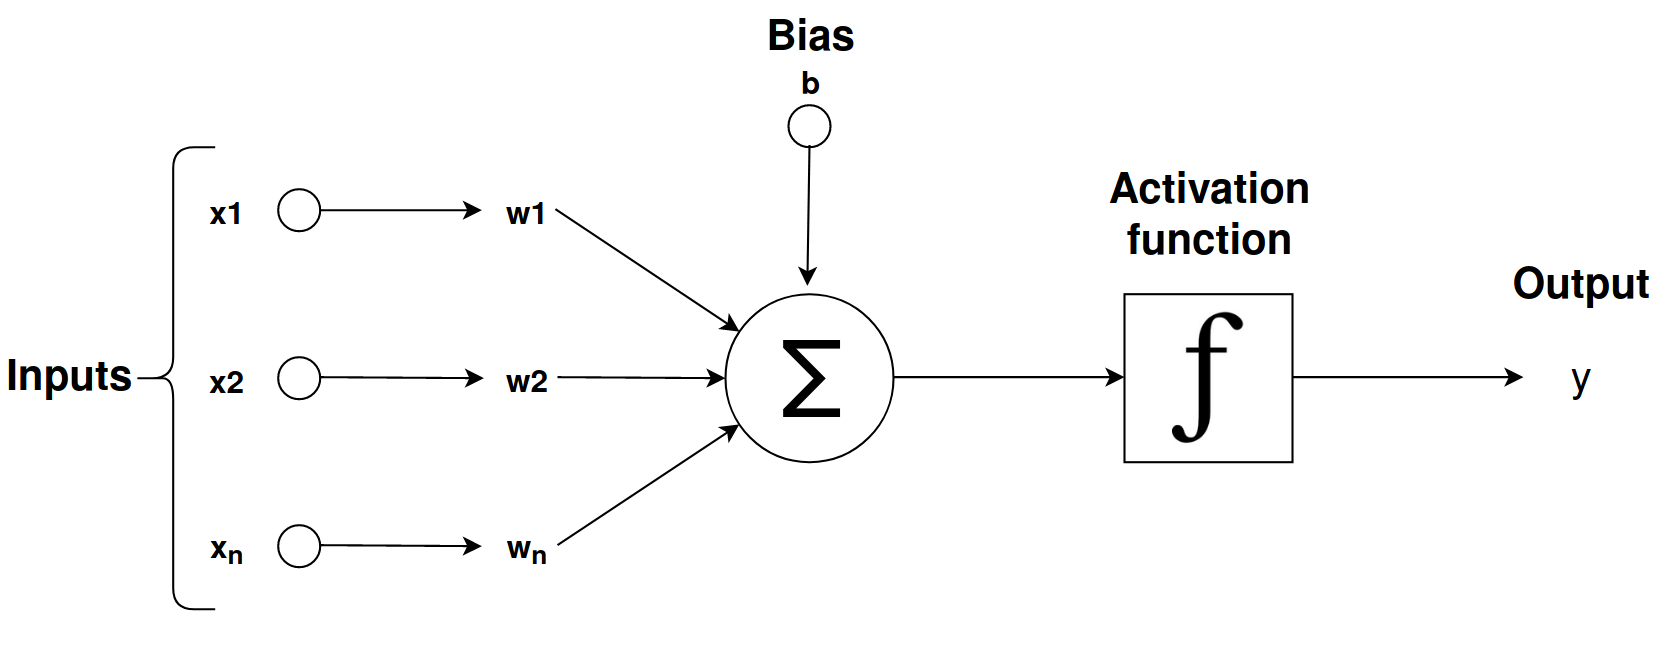
\includegraphics[scale = 0.15]{Sections/2StateOfTheArt/2_images/neuron.png}
        \caption{ Operations done by a neuron \cite{neuron}.}
        \label{fig:neuron}
    \end{figure}
    
    
   
    \par To put it simply, a neural network can be compared to a filter that goes through all of the possibilities, so that the computer is able to come up with the correct answer.
    \par Sometimes, an object might be too similar to another object which can make the network output a wrong answer. The solution to this problem is the usage of a back-propagation algorithm. This algorithm allows the network to adjust the connections back through the network, check if all the bias values are correct and all of the connections are weighted properly \cite{ArmaanMerchant2018}.
    


        \begin{itemize}
            \item \textbf{Neural Network Training}
        \end{itemize}
    \par The best way to train a neural network from scratch is to design a network architecture that will learn through the feeding of a large dataset of labeled data. This allows it it to learn the features and model. The problem with this is that depending on the learning rate of the network and the amount of data, these networks can take a lot of time to train (days, maybe weeks). 

    \par To solve the problem of time, deep learning applications can recur to the usage of transfer learning. Transfer learning is a process that involves the fine-tuning of a pretrained model. This works by using an existing network like GoogLeNet, and feed it new data of previously unknown classes to the network. After some tweaks to the network, it will be able to categorize only a specific object instead of many different ones. This not only allows the network to be more precise in categorizing that one specific object, but it will also save lot of computation time \cite{mathworks_deeplearning}.


 

%%%%%%%%%%%%%%%%%%%%%%%%%%%%%%%%%%%%%%%%%%%%%%%%%%%%%%%%%%%%%%%%%%%%%%%%%%%%%

    \section{Datasets With Common Objects}

    \label{dataset}

    \par A dataset is a collection of images and videos that contain every day life objects that are manually labeled. State-of-the-art object detection models require deep learning neural networks, and in order for neural networks to be trained, they  require training datasets, as previously explained.  

    \par A few examples of some available datasets are:  MS COCO \cite{Lin2014}, ImageNet \cite{Takamitsu1978} , VisualGenome \cite{Language2015}, OpenImages \cite{Kuznetsova2018} and Pascal-VOC \cite{Everingham2010}.

    \par Some of these datasets propose challenges, where teams are able to compete in order to achieve state-of-the-art results. This subject is discussed in section \ref{sec:state}
    %%%%%%%%%%%%%%%%%%%%%%%%%%%%%%%%%%%%%%%%%%%%%%%%%%%%%%%%%%%%%%%%%%%%%%%%%%%%%%%%%%

%%%%%%%%%%%%%%%%%%%%%%%%%%%%%%%%%%%%%%%%%%%%%%%%%%%%%%%%%%%%%%%%%%%%%%%%%%%%%


\section{Computer Vision Libraries}
\label{sec:libraries_cv}


%%%%%%%%%%%%%%%%%%%%%%%%%%%%%%%%%%%%%%%%%%%%%%%%%%%%%%%%%%%%%%%%%%%%%%%%%%%%%%%
    \begin{itemize}
        \item \textbf{OpenCV}
    \end{itemize}

    OpenCV is an open source computer vision and machine learning software library originally developed by Intel in the year 2000 \cite{Culjak2012}.\par

    The library has more than 2500 optimized algorithms, which includes a comprehensive set of both classic and state-of-the-art computer vision and machine learning algorithms. These algorithms can be used to detect and recognize faces, identify objects, classify human actions in videos, track camera movements, track moving objects, extract 3D models of objects, produce 3D point clouds from stereo cameras, stitch images together to produce a high resolution image of an entire scene, find similar images from an image database, remove red eyes from images taken using flash, follow eye movements, recognize scenery and establish markers to overlay it with augmented reality, etc. \cite{opencvweb} \par
    
    OpenCV Supports the deep learning frameworks like Tensorflow, Torch/PyTorch, Caffe and it is the most standardized tooling for computer vision.  

   \begin{itemize}
       \item \textbf{Tensorflow}
   \end{itemize} 

    \label{Tensorflow}
   

    Tensorflow is currently the most popular open source framework for numerical computation and large-scale machine learning introduced by google and was originally created for tasks with heavy numerical computations.  \cite{Abadi} \cite{Dignam1983} 
    
    Tensorflow is written in c++ which enables extremely fast compile times, non the less, it can still be accessed by other languages, such as Python and also supports CPUs, GPUs and distributed processing. \par
    

    The name given to tensorflow comes from the inputs, since it receives inputs as a multi-dimensional array, also known as tensors. The input (tensor) goes on one end and then it “flows” throughout a system of operations and comes out on the other end as output. \par 
    
    Tensorboard is a feature of tensorflow that allows the monitoring of what tensorflow is doing graphical and visually.\par

%%%%%%%%%%%%%%%%%%%%%%%%%%%%%%%%%%%%%%%%%%%%%%%%%%%%%%%%%%%%%%%%%%%%%%%%%%%%%  
    \begin{itemize}
        \item \textbf{VLFeat}
    \end{itemize}

    The VLFeat open source library implements popular computer vision algorithms specializing in image understanding and local features extraction and matching. Algorithms include Fisher Vector, VLAD, SIFT, MSER, k-means, hierarchical k-means, agglomerative information bottleneck, SLIC superpixels, quick shift superpixels, large scale SVM training, and many others. It is written in C for efficiency and compatibility, with interfaces in MATLAB for ease of use, and detailed documentation throughout. It supports Windows, Mac OS X, and Linux \cite{vedaldi08vlfeat}.

    \begin{itemize}
        \item \textbf{BoofCV}
    \end{itemize}

    BoofCV is an open source library written from scratch for real-time computer vision. Its functionality covers a range of subjects, low-level image processing, camera calibration, feature detection/tracking, structure-from-motion, fiducial detection, and recognition. \par
	This library is organized into several packages: image processing, features, geometric vision, calibration, recognition,visualize, and IO. Image processing contains commonly used image processing functions which operate directly on pixels. Features contains feature extraction algorithms for use in higher level operations. \par Calibration has routines for determining the camera's intrinsic and extrinsic parameters. Recognition is for recognition and tracking complex visual objects. Geometric vision is composed of routines for processing extracted image features using 2D and 3D geometry. Visualize has routines for rendering and displaying extracted features. IO has input and output routines for different data structures \cite{boofcvweb}.

    \begin{itemize}
        \item \textbf{GluonCV}
    \end{itemize}

    GluonCV is a toolkit that offers pre-trained models, performance metrics of the different available models, consistent interface for when switching between the models, regular re-training and continuous integration to ensure code correctness, detailed documentation and well-documented examples. It also supports a range of different applications like : image classification, object detection, semantic segmentation, instance segmentation, pose estimation, video action recognition, depth prediction and a few others.

   In short, gluonCV provides implementations of state-of-the-art deep learning algorithms in computer vision. It aims to help engineers, researchers, and students quickly prototype products, validate new ideas and learn computer vision \cite{Guo2019}.

    
%%%%%%%%%%%%%%%%%%%%%%%%%%%%%%%%%%%%%%%%%%%%%%%%%%%%%%%%%%%%%%%%%%%%%%%%%

    


\section{Recent Innovations and Improvements}
\label{sec:state}

\par Image classification and object detection are both subjects that are constantly innovating and improving upon previously results, every month new papers are published with new and more efficient networks. 
\par In the Figures \ref{fig:leaderboard_object} and \ref{fig:leaderboard_image} it is shown  not only the current best methods for both image classification and object detection but also the development of the state-of-the-art throughout the years.


\begin{figure}[H]
    \centering
    \captionsetup{justification=centering}
    \begin{subfigure}{0.49\textwidth}
        \includegraphics[width=\textwidth]{Sections/2StateOfTheArt/2_images/chart_object.pdf}
        \caption{Object Detection on COCO test-dev benchmark \cite{papers_object}}
        \label{fig:leaderboard_object}
        \end{subfigure}
        \begin{subfigure}{0.49\textwidth}
        \includegraphics[width=\textwidth]{Sections/2StateOfTheArt/2_images/chart_image.pdf}
        \caption{Image Classification on ImageNet benchmark \cite{papers_image}}
        \label{fig:leaderboard_image}
        \end{subfigure}
    \label{fig:example_f1}
\end{figure}




\par Due to the fact that object detection is a subject of great innovation, there is an extreme amount of papers that try to compete for the best results coming out every few months. So, in order to do a review of the state-of-the-art, the Tables \ref{table:cocotable} and \ref{table:imagenettable} show the benchmarks for both imageNet and COCO test-dev. These tables were obtained from \cite{Ribeiro} and are based on the analysis of \cite{papers_image} and \cite{papers_object} which is a website dedicated to  the current state-of-the-art for object detection and image classification.






\subsection{COCO Test-Dev}

\par The COCO benchmark \cite{Lin2014} is a dataset that places object recognition in the context of scene understanding. The evaluation metric used is the average precision (AP). Table \ref{table:cocotable} shows the current best architectures and their respective score for the COCO test-dev dataset.

\begin{table}[H]
    
    \centering
    \caption {COCO Test-Dev Benchmarks.}
    \begin{tabular}{| c | c | c | c ||} 
    \hline
    Method & Backbone & AP (\%)  \\ [0.5ex] 
    \hline\hline
    Liu et al.(2019) \cite{Liu2019}  & ResNeXt-152 & 53.3 \\ 
    \hline
    Tan et al. (2019) \cite{Tan2019} & EfficientNet & 51.0 \\
    \hline
    Zhang et al. (2019) \cite{Zhang2019} & ResNeXt-101 & 50.7
    \\
    \hline
    Girshick et al. (2018) \cite{Detectron2018} & ResNeXt-152 & 50.2
    \\
    \hline
    Li et al. (2019) \cite{Li2019} & ResNet-101 & 48.4
    \\ [1ex] 
    \hline
    Zhang et al. (2019) \cite{Zhang2019} & ResNet-101  & 46.3
    \\ [1ex]
    \hline
    Mahajan et al. (2018) \cite{Mahajan2018} & ResNeXt & 45.2
    \\ [1ex]
    \hline
    Zhao et al. (2019) \cite{Zhao2019} & VGG16 & 44.2
    \\ [1ex]
    \hline
    Cai et al. (2018) \cite{Cai2018} & ResNet-101 & 42.8
    \\ [1ex]
    \hline
    Wang et al. (2019) \cite{Wang2019} & ResNet-50    & 39.8
    \\ [1ex]
    \hline
    Lin et al. (2017) \cite{Lin2017} & ResNet-101 & 39.1
    \\ [1ex]
    \hline
    Shrivastava et al. (2016) \cite{shrivastava2016skip} & Inception-ResNet-v2 & 36.8
    \\ [1ex]
    \hline
    Kim et al. (2018) \cite{Kim2018} & VGG-16 & 35.2
    \\ [1ex]
    \hline
   \end{tabular}
   \label{table:cocotable}
\end{table}

\par Liu et al. \cite{Liu2019} achieved the best score in the COCO Test-Dev in 2019. They proposed better detection performance by creating a more powerful backbone network from previously existing backbones like ResNet \cite{He2016} and ResNetXt \cite{Xie2017}. They implemented a strategy for assembling multiple identical backbones (called Assistant Backbones and Lead Backbones) linked by composite connections between the adjacent backbones in order to form a more powerful backbone which was given the name of Composite Backbone Network (CBNet).

\par In typical CNN based detectors, the backbone network (the baseline of a network architecture) is used for basic feature extraction.

\par CBNet feeds the output features of the previous backbone as an input feature to the succeeding backbone through composite connections.At the final stage, the Lead Backbone outputs features for object detection.

\par This architecture was able to achieve the best result in the COCO Test-Dev with a 53.3\% AP with single model by integrating a CBNet using triple ResNeXt-152 \cite{Xie2017} backbones into the Cascade Mask R-CNN baseline.


\par Figure \ref{fig:cbnet} presents the architecture for CBNet.



\begin{figure}[H]
    \centering
    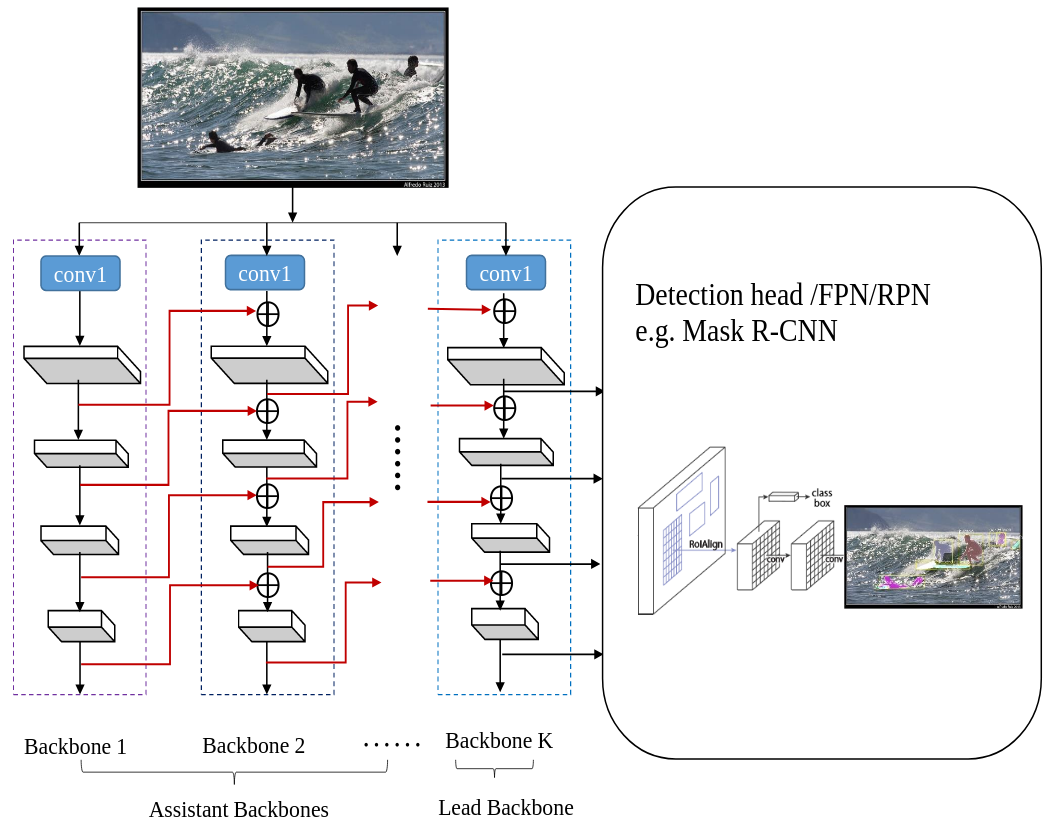
\includegraphics[scale = 0.25]{Sections/2StateOfTheArt/2_images/cbnet.png}
    \caption{CBNet Architecture for object detection \cite{Liu2019}.} 
    \label{fig:cbnet}
\end{figure}


\begin{itemize}
    \item \textbf{ResNeXt}
\end{itemize}

\label{sec:resnext}
\par ResNeXt, also known as Aggregated Residual Transform Network was created by facebook researchers and it is a simple highly modularized network architecture for image classification. 
\par The network is constructed by repeating a building block that aggregates a set of transformations with the same topology. The simple design results in a homogeneous, multi-branch architecture that has only a few hyper-parameters to set. This strategy creates a new dimension, which was given the name of "cardinality" (size of the set of transformations). 
\par This architecture is an improvement over the Inception architectures, being more simple in design and adding more branches (towers) within modules. \cite{Xie2017}


\begin{figure}[htb]
    \centering
    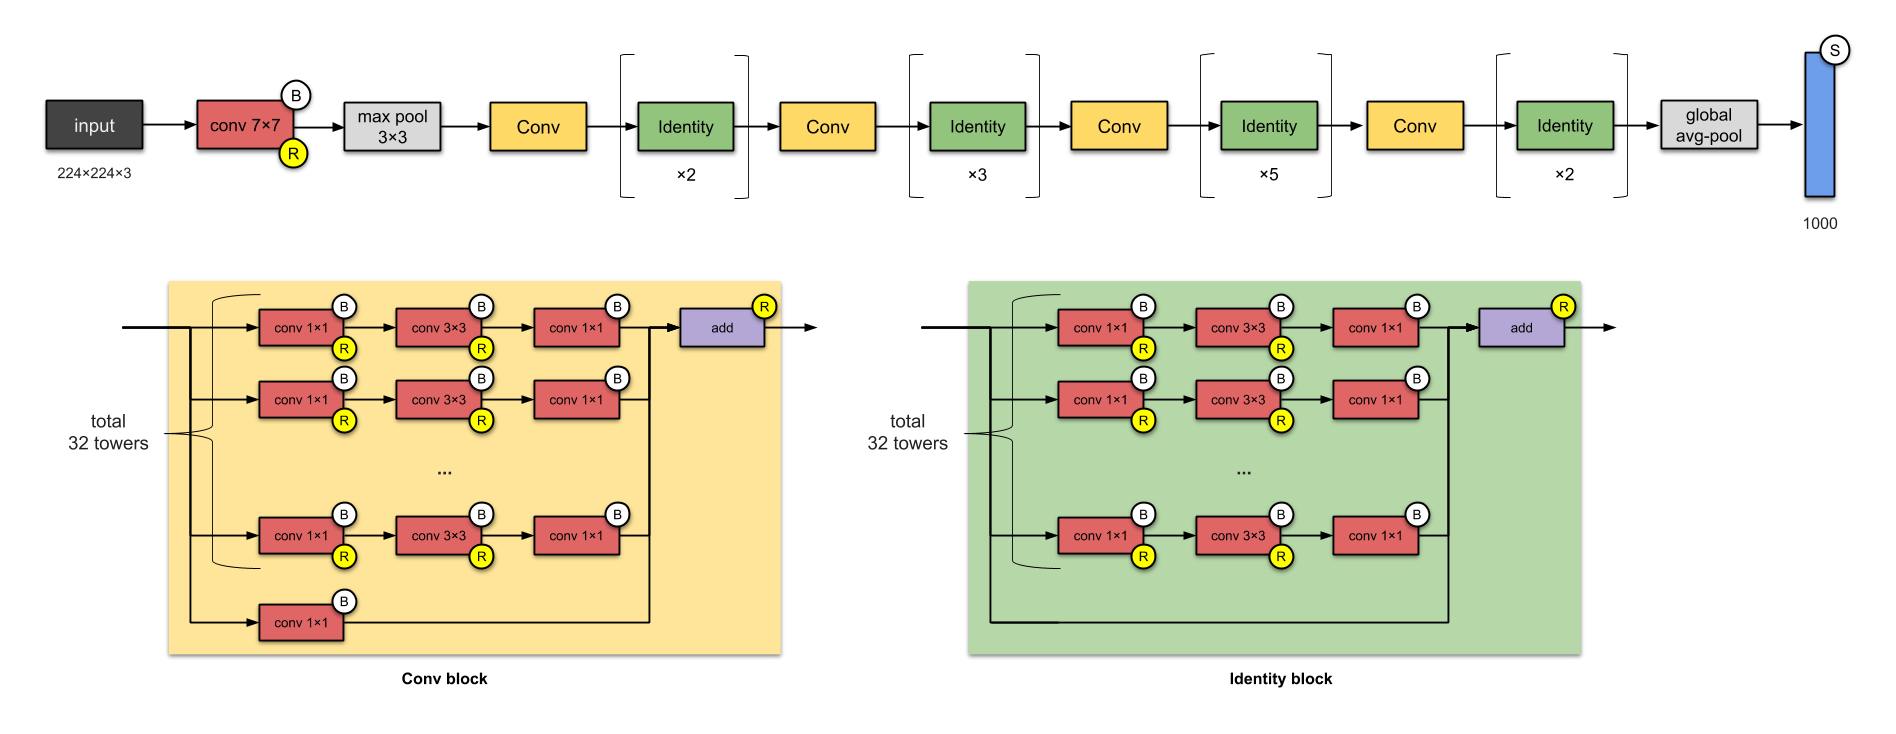
\includegraphics[scale = 0.23]{Sections/2StateOfTheArt/2_images/resnext.png}
    \caption{ResNeXt architecture \cite{cnnarchitectures}. }
    \label{fig:noisestudent}
\end{figure}


\newpage

\subsection{ImageNet}
\par The imageNet Large Scale Visual Recognition challenge \cite{Russakovsky2015} is a benchmark for object category classification and detection. The evaluation metrics used are top-1 and top-5 accuracy.

\begin{table}[htb]
    
    \centering
    \caption {ImageNet Benchmarks.}
    \begin{tabular}{|| c | c | c ||} 
    \hline
    Method & Backbone & Top-1 Acc (\%)  \\ [0.5ex] 
    \hline\hline
    Xie et al. (2019) \cite{Xie2019}& EfficientNet & 88.4
    \\ 
    \hline
    Kolesnikov et al. (2019) \cite{alex2019large} & ResNet-152 & 87.8

    \\
    \hline
    Touvron et al. (2019) \cite{touvron2019fixing} & ResNeXt-101 & 86.4

    \\
    \hline
    Xie et al. (2019) \cite{xie2019adversarial} & EfficientNet & 85.5

    \\ [1ex] 
    \hline
    Mahajan et al. (2018) \cite{Mahajan2018} & ResNeXt & 85.4

    \\ [1ex]
    \hline
    Tan et al. (2019) \cite{tan2019efficientnet}& EfficientNet & 84.4

    \\ [1ex]
    \hline
    Touvron et al. (2019) \cite{touvron2019fixing} & ResNet-50 & 82.5

    \\ [1ex]
    \hline
    Szegedy et al. (2017) \cite{szegedy2016inceptionv4} & Inception-resnet-v2 & 80.1

    \\ [1ex]
    \hline
    Szegedy et al. (2017) \cite{szegedy2016inceptionv4}  & Inception-v4 & 80.0

    \\ [1ex]
    \hline
    Simonyan et al. (2014) \cite{simonyan2014deep} & VGG-16 & 74.4
    \\ [1ex]
    \hline
   \end{tabular}
   \label{table:imagenettable}
\end{table}



\par Xie et al. \cite{Xie2019} stated that current state-of-the-art vision models are still trained with supervised learning, which implies the necessity of large corpus of labeled images in order to work properly. The fact that current models are only shown labeled images causes an obvious limitations in the improvement of accuracy and robustness of current state-of-the-art models, this can be improved with the usage of the large available quantities of unlabeled images available.
\par Having this in mind, they decided to use unlabeled images to improve the state-of-the-art ImageNet accuracy and show that accuracy has an outsized impact on robustness. For this purpose, they used a much larger corpus of unlabeled images, where a large fraction of images did not belong to ImageNet training set distribution.
\par Using a self-training framework the model was trained with 3 main steps which consist in:

\begin{enumerate}
    \item Training of a teacher model on labeled images.
    \item Usage of the teacher to generate pseudo labels on unlabeled images.
    \item Train a student model on the combination of labeled images.
\end{enumerate}

\par The algorithm was iterated a few times by treating the student as a teacher to relabel the unlabeled data and training a new student.

\par An important discovery was made during the training of the algorithm. For the method to work well at scale the student model should be noised during its training while the teacher should not be noised during the generation of pseudo labels. This way, the pseudo labels are as accurate as possible and the noised student is forced to learn harder from the pseudo labels. To induce noise in the model it was used RandAugment data, dropout and stochastic depth during the training. Figure \ref{fig:noisestudent} shows a brief view of how the method works.
\par This is where the name of the method "Noisy Student"comes from, since the student is noised to learn beyond the teacher's knowledge.
\par With this method they were able to show that it is possible to use unlabeled images to significantly advance both accuracy and robustness of state-of-the-art imageNet models.
\par The presented model uses EfficientNe as a backbone trained on images from imageNet dataset and was able to obtain the best results in the ImageNet benchmark dataset by achieving an accuracy of 88.4\%.



\begin{figure}[htb]
    \centering
    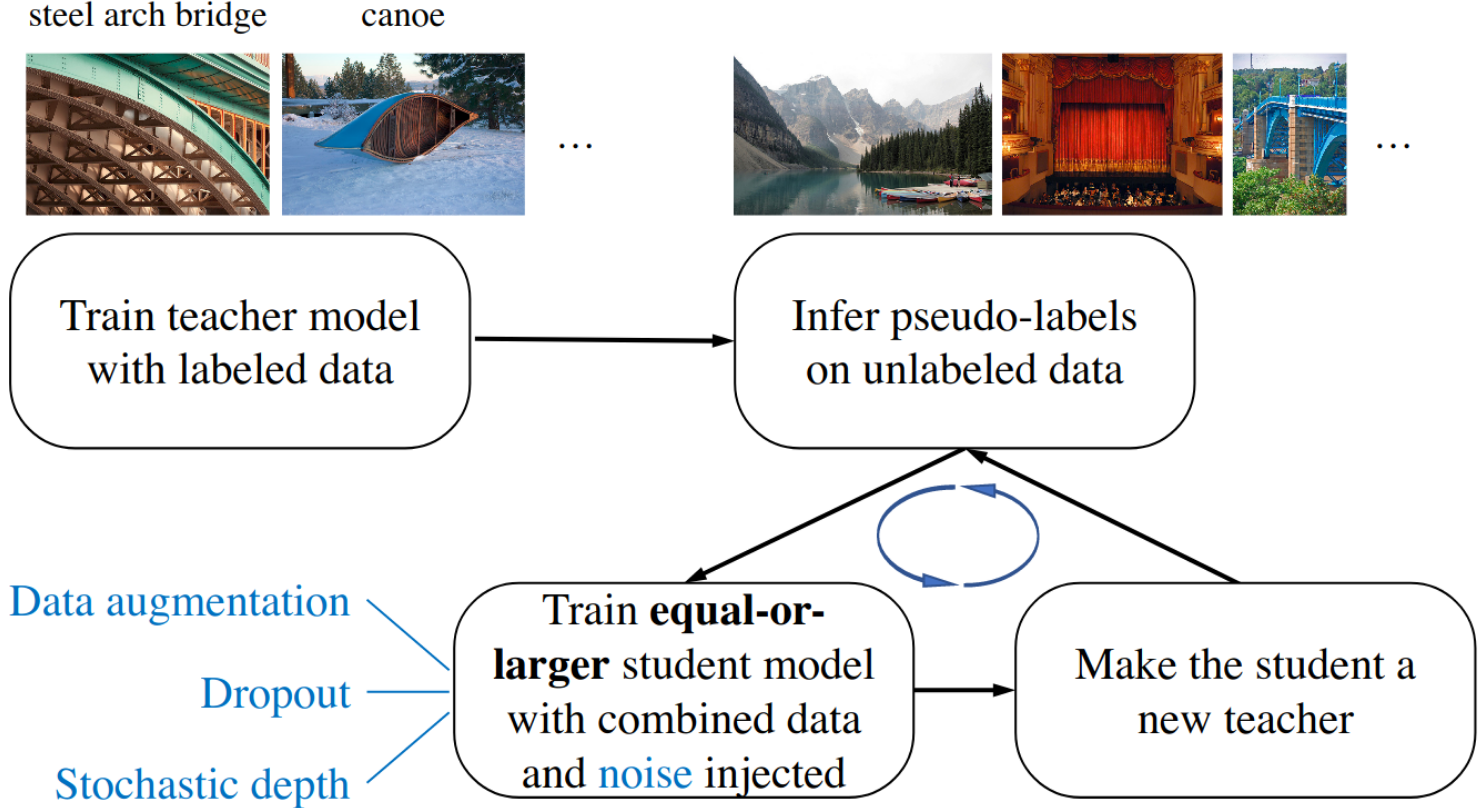
\includegraphics[scale = 0.15]{Sections/2StateOfTheArt/2_images/noisy_student.png}
    \caption{Noisy Student Method \cite{Xie2019}.} 
    \label{fig:noisestudent}
\end{figure}cnnarchitectures

\par Researchers at Google decided to study the impact of scaling up CNNs, in order to achieve better accuracy and efficiency. EfficientNet-B0 was developed based on a simple idea, scaling each of the dimensions of the network (width, depth and resolution) with a constant ratio, improves the overall performance \cite{tan2019efficientnet}.

\begin{figure}[htb]
    \centering
    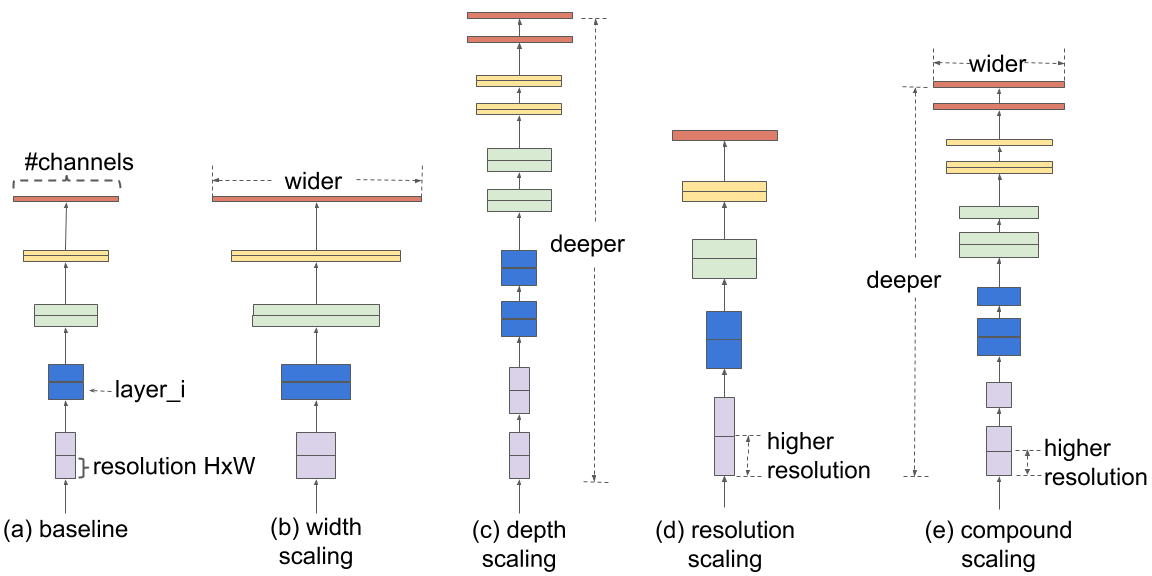
\includegraphics[scale = 0.25]{Sections/2StateOfTheArt/2_images/efficientNet_scale.png}
    \caption{Comparison of different scaling methods:  (a) is a baseline network example; (b)-(d) are conventional scaling that only increases one dimension of network  width, depth, or resolution. (e) is the proposed compound scaling method that uniformly scales all three dimensions with a fixed ratio \cite{tan2019efficientnet}.
    } 

\end{figure}

\newpage

\par The baseline network architecture, EffecientNet-B0, uses mobile inverted bottleneck convolution (MBConv), similar to MobileNetV2 \cite{s2018mobilenetv2} and MnasNet \cite{tan2018mnasnet}. Figure \ref{fig:eff} shows the baseline network architecture EfficientNet-B0.

\begin{figure}[htb]
    \centering
    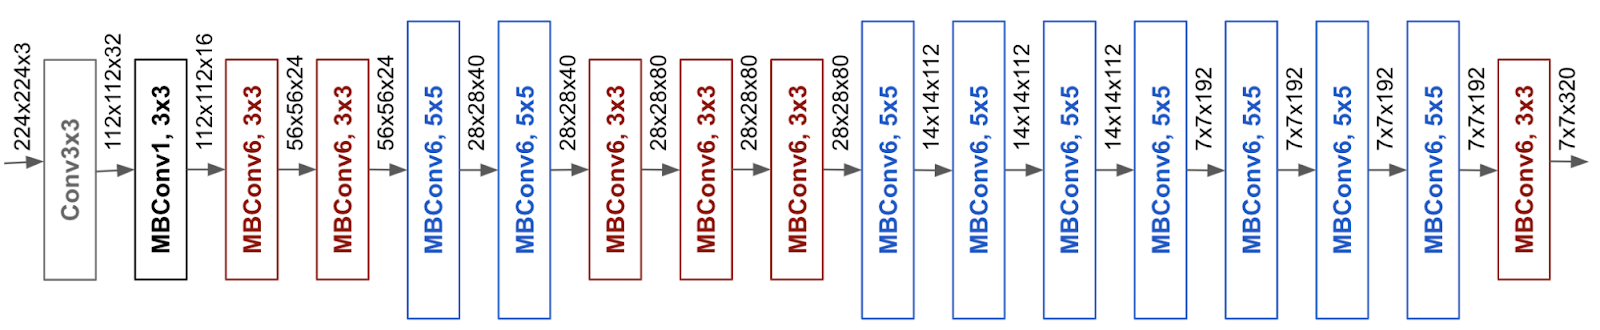
\includegraphics[scale = 0.22]{Sections/2StateOfTheArt/2_images/efficientNet_Arch.png}
    \caption{EfficientNet-B0 architecture representation \cite{Tan}.} 
    \label{fig:eff}

\end{figure}


\section{Final Remarks}


The models and algorithms experimented in this thesis were provided trough a computer vision python library called imageAI, which allows the ability to easily use state-of-the-art AI features \cite{ImageAI}. This library required the pre-installation of TensorFlow, OpenCV and Keras libraries. The Keras library \cite{CholletFrancois2015} is an open-source neural-network library written in Python which is capable of running on top of TensorFlow.

During the development of the automatic retrieval system many of the described algorithms and models in Appendix \ref{ch:appendix} were tried. For image classification the algorithms tested were DenseNet, InceptionV3, ResNet and SqueezeNet. For object detection the models used were YoloV3, TinyYoloV3, RetinaNet and ResNetXt-101. The testing of all of these models was done in order to find the most suitable model to process the imageCLEF images dataset.

\cleardoublepage


\chapter{Information Extraction From Text}
\label{ch:nlp}

As previously discussed, the problem of big data has become more relevant in the recent years.  This problem does not apply only to the ever growing amount of multimedia data created by smartphones but also to the growing presence of information in the form of news, corporate files, medical records, government documents, court hearing and social media. There is an ever increasing flood of information in an unstructured form. Natural Language Processing (NLP) is related to the usage of computation methods to process such data as a mode of communication used by humans.

``There are lot many processes involved in the pipeline of NLP. At the syntactic level, statements are segmented into words, punctuation (i.e.  tokens) and each token is assigned with its label in the form of noun, verb, adjective, adverb and so on (Part of Speech Tagging).  At the semantic level, each word is analyzed to get the meaningful representation of the sentence.  Hence, the basic task of NLP is to process the unstructured text and to produce a representation of its meaning.''  \cite{singh2018natural}.



Information Extraction (IE) from text is the process of extracting useful information from textual sources by implementing techniques of NLP. It can be defined as the act of efficiently and effectively analyze text and extract valuable and relevant knowledge from it in the form of structured information. ``The goal of IE is to extract salient facts about pre-specified types of events, entities, or relationships, in order to build more meaningful, rich representations of their semantic content, which can be used to populate databases that provide more structured input.'' \cite{singh2018natural}.

In this thesis, NLP is implemented to serve the purpose of creating an algorithm capable of extracting relevant information from a textual source. Furthermore, the algorithm must also be able to categorize the extracted data according pre-specified categories such as "locations" and "activities".

This chapter starts with an introduction to Natural Language Processing in Section \ref{sec:nlp}. Section \ref{sec:num} explains the process of representing text in a numerical vector form while describing the concept of word embeddings. Static and contextualized word embedding models are introduced in Section \ref{sec:static} and \ref{sec:context} respectively. An overview on some of the available NLP libraries is presented in Section \ref{sec:libraries}. Finally, Section \ref{sec:final_remarks} gives the final remarks of this chapter.

\newpage
\section{Natural Language Processing}
\label{sec:nlp}

Natural language processing is a subfield of linguistics, computer science, information engineering and artificial intelligence, which is devoted to the engineering of computational models and processes to give the ability of human-like comprehension of texts/languages to computers. \cite{Khurana2018}  

Human language is extremely complex and rarely precise, to understand it is not only understand what words alone mean, but also how linking them together creates meaning. The nature of the human language makes NLP one of the most difficult tasks in computer science. 

Figure \ref{fig:nlp_class} shows the classification of NLP, which consists in two major components, Natural Language Understanding (NLU) and Natural Language Generation (NLG) \cite{Khurana2018}.  \par




\begin{figure}[htb]
    \centering
    \captionsetup{justification=centering}
    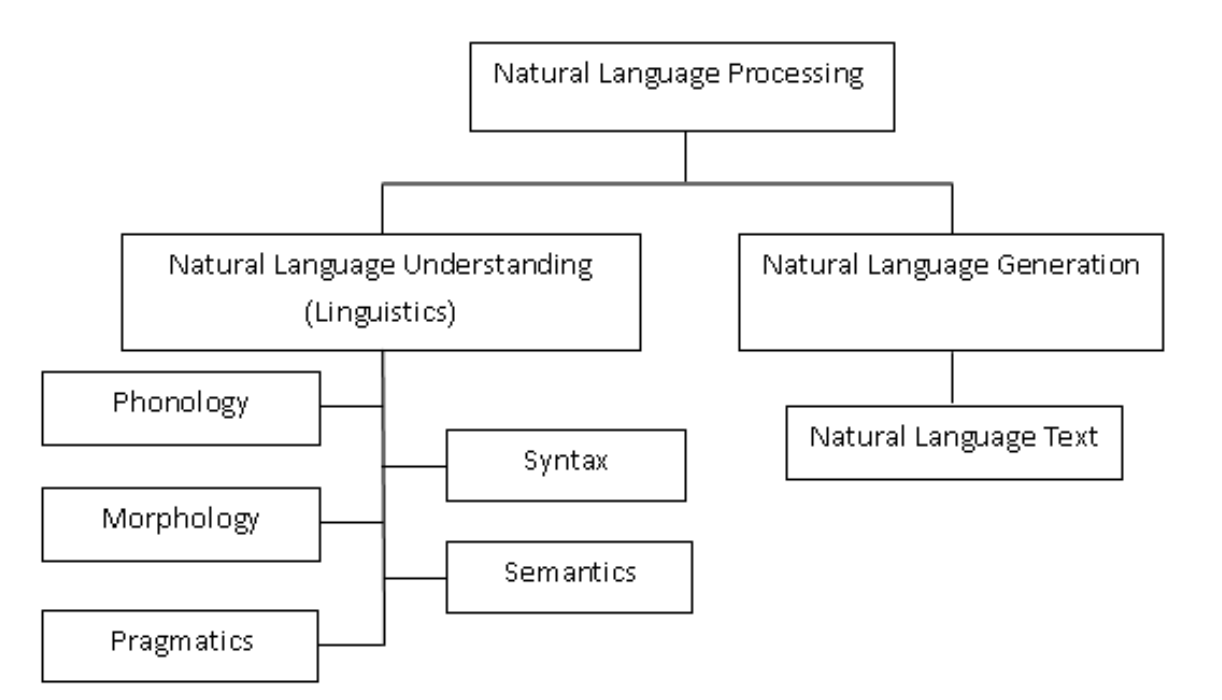
\includegraphics[width=0.7\textwidth]{Sections/3StateOfTheArt/3_images/NLP_diagram.png}
    \caption[Classification of NLP.]{Classification of NLP \cite{Khurana2018}.}  
    \label{fig:nlp_class} 
\end{figure}

Natural Language Understanding is the process of understanding text. It is related to the science of Linguistic that studies the meaning of languages, context and various forms of language. 

Natural Language Generation is the process of generating text, sentences and
paragraphs that are meaningful from an internal representation \cite{Khurana2018}. 

Using the visual representation of Figure \ref{fig:nlp_class} the important terminologies of NLP are as follows \cite{Khurana2018} :

\begin{itemize}
    \item \textbf{Phonology}: The part of Linguistics which refers to the systematic arrangement of sound;
    \item \textbf{Morphology}: In linguistics, morphology is the study of words, how they are formed, and their relationship to other words in the same language. The different parts of the word represent the smallest units of meaning known as Morphemes;
    \item \textbf{Lexical}: In Lexical the focus is the interpretation of the meaning of individual words;
    \item \textbf{Syntax}: Syntax refers to the study of the grammatical structure of the sentence;
    \item  \textbf{Semantic}: Semantic processing determines the possible meanings of a
    sentence by pivoting on the interactions among word-level meanings in the sentence;
    \item \textbf{Discourse}: Discourse focuses on the properties of the text as a whole that convey meaning by making connections between component sentences;
    \item \textbf{Pragmatic:}: Subfield of linguistics that studies the ways in which the context of a sentence contributes to the meaning. 
    
\end{itemize}

The field of NLP can be divided in two broad sub-areas: core areas and application areas. The core areas address fundamental problems such as language modeling, morphological processing, parsing and semantic processing \cite{Otter2018}. 



\begin{itemize}
    \item Language modeling is considered the most important task in NLP and an essential piece in any application of NLP. It is the process of creating a model capable of predicting words or simple linguistic components given previous words or components. It can capture syntactic and semantic relationships among words or components in a linear neighborhood, making it useful for tasks such as machine translation and text summarization.
    \item Morphological processing is the process of finding segments within single words,  including roots and stems, prefixes and suffixes.
    \item Parsing examines how different words and phrases relate to each other.
    \item Semantic processing is the task of understanding of the meaning of words and phrases. This is done recurring to  word embedding models, like Word2Vec. This will be further discussed in this chapter.
\end{itemize}





The application areas address topics such as extraction of useful information from text (e.g named entities and relations), translation of text, summarization of written documents, automatic answering of questions, chat bots, email spam detection and many others \cite{Otter2018}.




\section{Numerical Representation of Text}
\label{sec:num}

\par Machine learning algorithms and most of all deep learning architectures are incapable of processing strings of text, this is because they require numbers (vectors) as an input in order to perform linear algebra operations \cite{Vidhya2017} which is not possible with words. A human can easily tell that the word "dog" and the word "cat" are identical, since they both represent an animal, however a computer would assume that they are completely different things since all the letters in those  words are different. 

    \subsection{Word Embeddings}

    \par The dominant approach to solve this problem is the usage of word embeddings, which is a type of word representation that allows words with similar meaning to have a similar representation by mapping a set of words, or phrases in a vocabulary, to vectors of numerical values. For example, the word “happy” can be represented as a vector of 4 dimensions [0.24, 0.45, 0.11, 0.49] and “sad” has a vector of [0.88, 0.78, 0.45, 0.91]. The reason for this vectors to exist is so that a machine learning algorithm can perform linear algebra operations on numbers (vectors) instead of words \cite{MuratMustafa}. Word embedding methods learn a real-valued vector representation for a predefined fixed size vocabulary from a corpus  of text \cite{Brownlee2017}.A vector representation of a word may be a one-hot encoded vector where 1 stands for the position where the word exists and 0 everywhere else. 
    
    \par As an example, the sentence ”Word Embeddings are Word converted into numbers” can be converted to the following dictionary using the one-hot encoded vector representation : [‘Word’,’Embeddings’,’are’,’Converted’,"Word",’into’,’numbers’]. Using this representation the word “numbers” in the one-hot encoded vector is [0,0,0,0,0,1] and for the word "converted" is [0,0,0,1,0,0]. This is considered to be the most simple method to represent words in vector forms \cite{Vidhya2017}.

    \par The following image showcases the given example.
    
    
    \begin{figure}[htb]
        \centering
        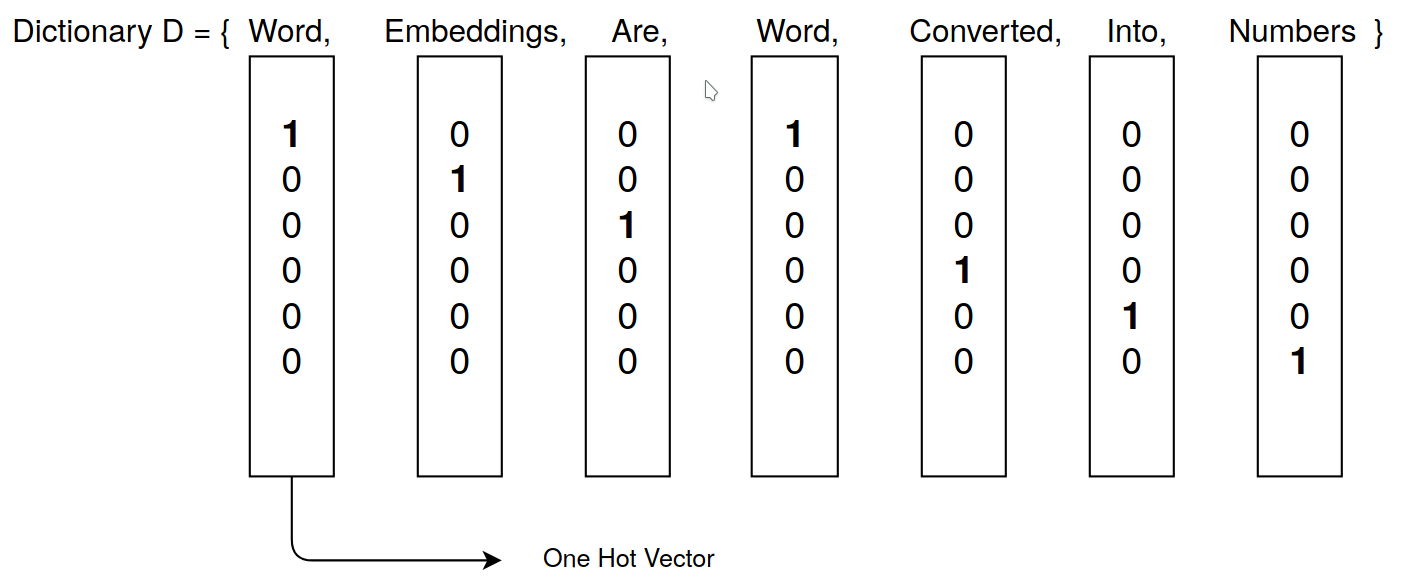
\includegraphics[scale = 0.23]{Sections/3StateOfTheArt/3_images/one_hot_encoding.png}
        \caption{Example of text representation by one-hot vector.}   
    \end{figure}
    
    
    



    \section{Static Word Embedding Models}
    \label{sec:static}

    \par This section introduces some common static word embedding models to learn word embeddings from text.


    \par Static word embedding have the fundamental problem which is they generate the same embedding, in different contexts, for the same word and once learned they do not change it. They map each word type to a single vector, making it harder to deal with the polysemy problem. This is due to the fact that each word has a single vector, regardless of context \cite{Mikolov2013}. Therefore, these models assume that the meaning of any given word is the same across the entire text.
   

    \par As an example, having these two phrases:

    \begin{itemize}
        \item "I saw her at the library."
        \item "Pass me the saw to cut the log in half."
    \end{itemize}

    \par In this case, the word "saw" has two different meanings. In the first phrase the word "saw" refers to the verb "see" and for the second phrase it refers to the tool "saw". However, for static word embedding models, words only have one single meaning and therefore  the word representation for "saw" would be the same in both cases.

    Dynamic word embeddings models represent “saw” differently according to the contexts, while static embedding can not distinguish the semantic difference between two “saws” and represent with the same vector no matter the context \cite{Wang2020} \cite{Batista2018}.

   
        \subsection{Word2Vec}

        One of the most important and most popular models developed in NLP was Word2Vec. Created by Tomas Mikolov, et al. \cite{Mikolov2013} at Google in 2013, Word2Vec is a two-layer neural network that processes text by "vectorizing" words with the purpose of grouping vectors of similar words together in vectorspace. These similarities are detected by creating vectors that are distributed numerical representations of word features, without human intervention. A vocabulary is outputted from Word2Vec where each item has a vector attached to it. This can be fed into a deep-learning network or queried to detect relationships between words, like similarities. The similarities are measured trough a cosine similarity, having no similarity is expressed as a cosine similarity of 0 since it is 90 degree angle, while a full similarity is expressed as cosine similarity of 1 and it is a 0 degree angle, complete overlap. Sweden is equal to Sweden therefore the cosine similarity is equal to 1, while Norway has a cosine distance of 0.760124 from Sweden \cite{Wiki}.
        
        


        In a regular one-hot encoded vector all words have the same distance between each other, even though their meanings are completely different, this creates a lost in information at the encoding.  However, Word2Vec is capable of learning vectors by understanding the context in which words appear. This results in vectors in which words with similar meanings end up with a similar numerical representation in the vectorspace. Figure \ref{fig:one_vs_word2vec} illustrates this situation. For instance, cats and dogs are more similar than fish and sharks. This extra information is useful for machine learning algorithms \cite{word2vec_explained}.	


        \begin{figure}[H]
            \centering
            \captionsetup{justification=centering}
          
            \begin{subfigure}{0.32\textwidth}
            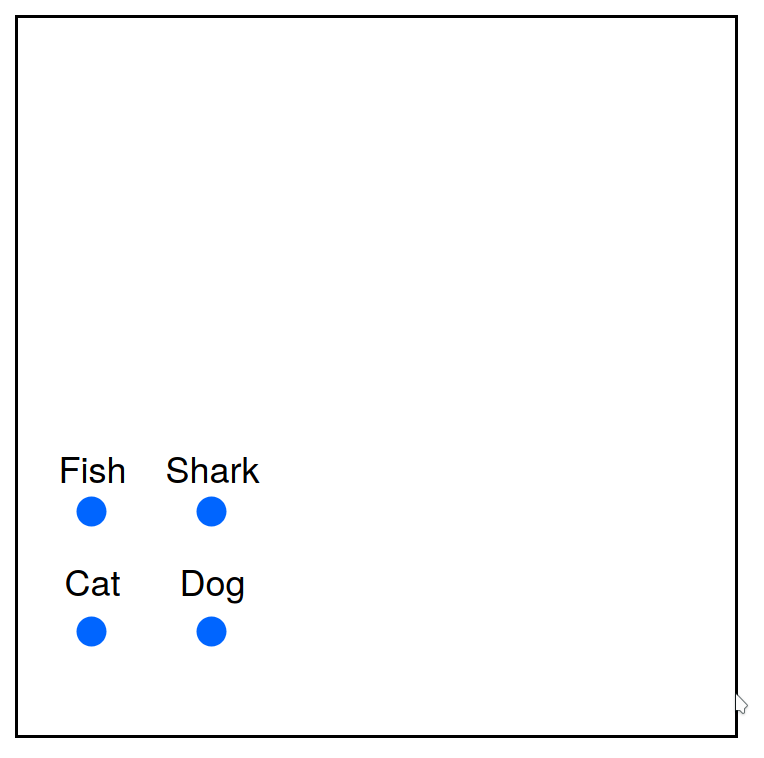
\includegraphics[width=\textwidth]{Sections/3StateOfTheArt/3_images/one_hot_ex.png} 
            \caption[One-hot encoding resulting vector.]{One-hot encoding resulting vector \cite{word2vec_explained}. }
          
            \end{subfigure}
            \begin{subfigure}{0.32\textwidth}
            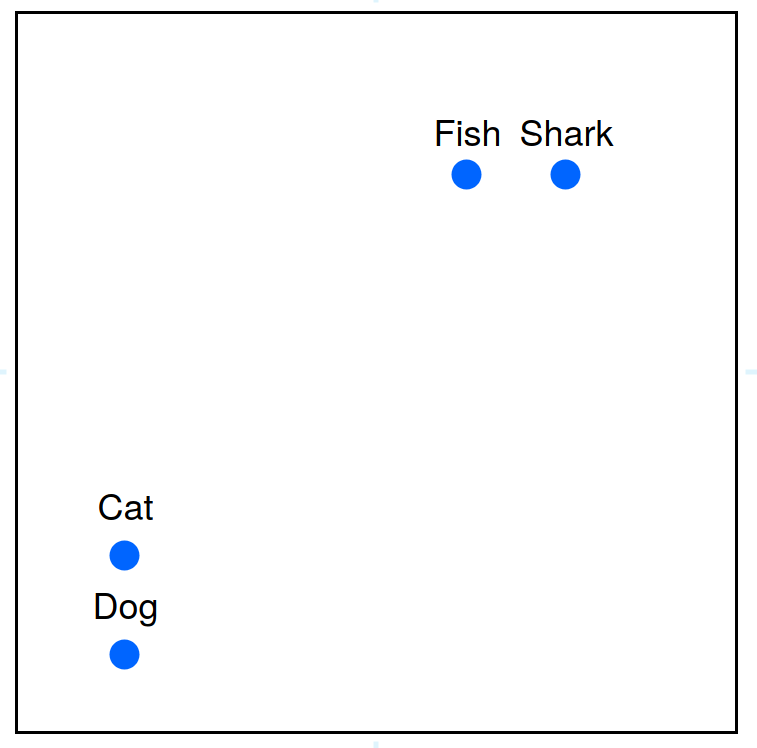
\includegraphics[width=\textwidth]{Sections/3StateOfTheArt/3_images/word2vec_encode.png}\hfill
            \caption[Word2Vec encoding resulting vector]{Word2Vec encoding resulting vector \cite{word2vec_explained}. }
            \end{subfigure}
            \caption{}
            \label{fig:one_vs_word2vec}

          \end{figure}

          Furthermore, using a word offset technique, Word2Vec is capable of performing simple algebraic operations to the word vectors. An example is that the vector(”King”) - vector(”Man”) + vecs
          tor(”Woman”) results in a vector that is closest to the vector representation of the word "Queen" \cite{Mikolov2013}. 

        
        Word2Vec is composed of two different models, CBOW (Continuous Bag of words) which predicts a word given the context and Skip-Gram which predicts context given a word \cite{Mikolov2013} \cite{Wiki} as shown in Figure \ref{fig:cbow_skip}.

        

        \begin{figure}[H]
            \centering
            \captionsetup{justification=centering}
            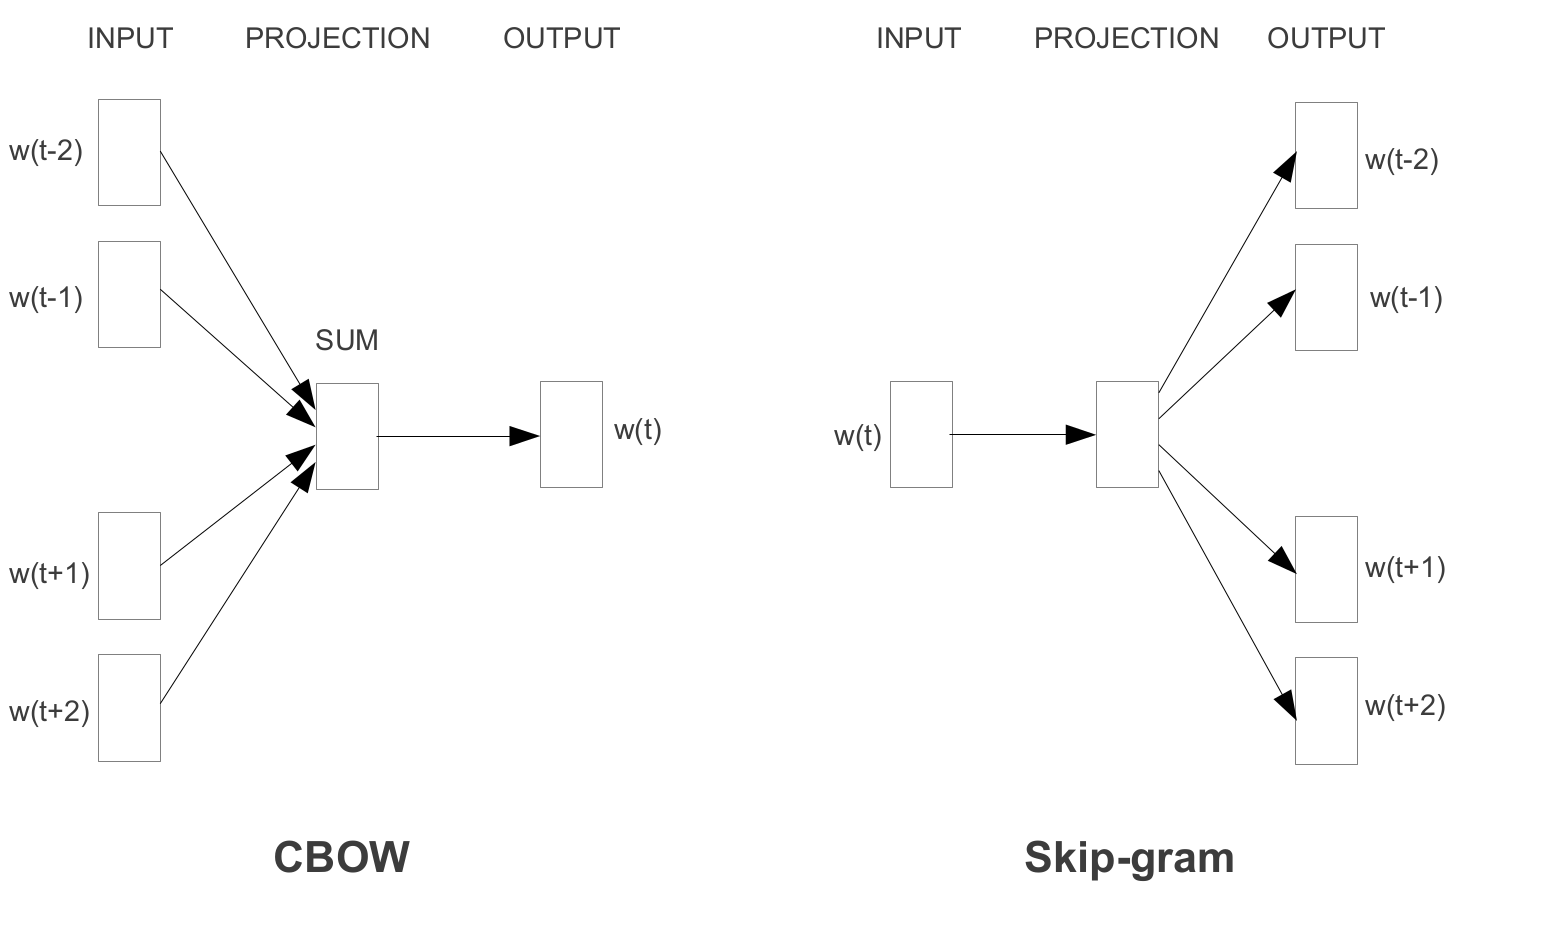
\includegraphics[width=0.8\textwidth]{Sections/3StateOfTheArt/3_images/Cbow_Skip.png}
            \caption[CBOW and Skip-gram models]{CBOW and Skip-gram models \cite{Mikolov2013}.} 
            \label{fig:cbow_skip}
        \end{figure}



        \begin{itemize}
            \item \textbf{Continuous Bag of Words}
        \end{itemize}


       CBOW allows to take a big amount of text and train a neural network to predict a word inputting the N words at each side. In the given example in Figure \ref{fig:cbow_skip}  N = 2. Using the example given in \cite{Mordecki2017} : “The monkey is eating a banana”, the word "eating" is predicted given that the previous two words are "The" and "monkey" and the next two are "a" and "banana".

        Using Figure \ref{fig:cbow_skip} again, the inputs of CBOW would be : w(t+2) = "monkey", w(t+1) = "is", w(t-1) = "a", w(t+2) = "banana" and the output (prediction) would be w(t) = "eating" \cite{Mordecki2017}.
        
        
        \begin{itemize}
            \item \textbf{Skip-gram}
        \end{itemize}

        Skip-gram is much identical to CBOW but instead of predicting a word given the context, it predicts the context given a word. 

        One again using Figure \ref{fig:cbow_skip}, the input of Skip-gram is w(t) = "eating" and the outputs would be : w(t+2) = "monkey", w(t+1) = "is", w(t-1) = "a", w(t+2) = "banana" \cite{Mordecki2017}.


        
        \subsection{GloVe}
            \par GloVe stands for Global Vectors for Word Representation and was a new approach created by Pennington et all. in 2014 \cite{Pennington2014} to generate word embeddings with unsupervised learning. Glove main goals are to create word vectors that capture meaning in the vector space and to take advantage of global count statistics instead of using only local information. 
            \par The problem with Word2Vec is that it only takes local information into account, and does not consider global context. This means that the semantics learnt for a given word are only affected by the surrounding words. 
            \par GloVe works by aggregating global word-to-word co-occurrence matrix from a of corpus text. This means that if two words keep appearing together in a corpus of text they either share a linguistic or a semantic similarity. Simply put, similar words will be placed together in the high-dimensional space. Therefore GloVe can be seen like an extension to the Word2Vec model.

        \subsection{FastText}

        \par FastText, created by Facebook's AI Research (FAIR) lab in 2016, is a fast text classifier based on the skipgram model  used for efficient learning of word representations and sentence classification. Popular models like word2Vec and GloVe  are based on continuous word representations that create vectors directly from words in a sentence while ignoring the morphology of words, this is done by assigning a distinct vector to each word, fastText uses a different approach treating each word as bag of characters n-grams. A vector representation is associated to each character n-gram and words are represented as the sum of these representations. This allows fastText to work with rare words not seen in the training data since the word is broken down into n-grams to get the corresponding embeddings \cite{bojanowski2016enriching}.


        \par Using the word "where" as an example and n=3, the representation of this word in a fastText model is <wh, whe, her, er, re> and the special sequence <where>. The angular brackets serve as boundary symbols to distinguish the n-gram of a word from the word itself, this means that if the word "her" was part of the vocabulary it would be represented as <her>, which allows the preservation of the meaning of shorter words and the understanding of suffixes and prefixes.

        

    
    \section{Contextualized Word Embedding Models}
    \label{sec:context}    
        \par Contextualized words embeddings aim at capturing word semantics in different contexts to address the issue of polysemous and the context-dependent nature of words \cite{Batista2018}. Using the example given in  Section \ref{sec:static}, these models would be able to distinguish the different meaning of the word "saw" given the two different sentences.

        \subsection{Context2vec}
        
            \par Context2Vec is an unsupervised model capable of learning efficiently generic context embedding of wide sentential contexts, using a bidirectional LSTM. 

            A large plain text corpora is utilized in order to learn a neural model capable of embedding  entire  sentential  contexts  and  target words in the same low-dimensional space, which is optimized to reflect inter-dependencies between targets and their entire sentential context as a whole. 
            
            
            In contrast to word2vec that use context modeling mostly internally and considers the target word embeddings as their main output, the focus of context2vec is the context representation. Context2vec achieves its objective by assigning similar embeddings to sentential contexts and their associated target words \cite{Melamud2016}.

            \begin{figure}[H]
                \centering
                \captionsetup{justification=centering}
                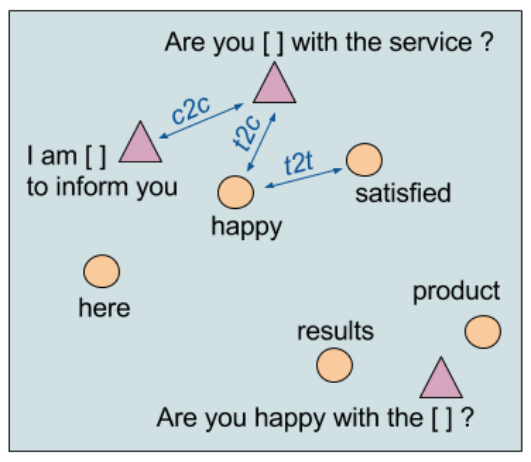
\includegraphics[width=0.4\textwidth]{Sections/3StateOfTheArt/3_images/context2vec_embedding.png}
                \caption[Context2vec’s embedded space and similarity metrics.]{A 2D illustration of context2vec’s embedded space and similarity metrics. Triangles and circles denote sentential context embeddings and target word embeddings, respectively \cite{Melamud2016}.} 
            \end{figure}

            \begin{figure}[H]
                \centering
                \captionsetup{justification=centering}
                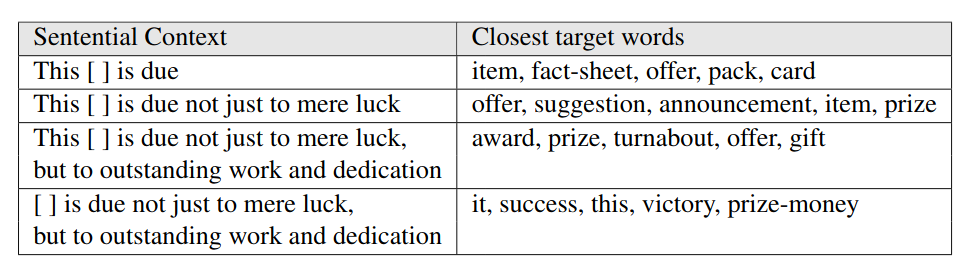
\includegraphics[width=0.8\textwidth]{Sections/3StateOfTheArt/3_images/context2vec_predict.png}
                \caption[Context2vec's closest target words]{Closest target words to various sentential contexts, illustrating context2vec’s sensitivity to long range dependencies, and both sides of the target word \cite{Melamud2016}.} 
            \end{figure}
            
        \newpage


        \subsection{ELMo}

            \par ELMo (Embeddings from Language Models) is a NLP model with context-aware representation, it understands different meanings for the same word since it takes into account the surrounding words unlike traditional word embedding models such as Word2Vec and GLoVe. In order to achieve this, ELMo attributes an embedding for each word after looking at the entire context in which it is used, instead of using fixed embeddings for each word. Therefore, the same word might have different word vectors under different contexts.
            \par This NLP models both syntax and semantics of word use and how these uses vary across linguistic context.The word vectors are learned through the usage of internal states of a deep bidirectional LSTM algorithm, trained on a large corpus of text. Bidirectional implies that the algorithm takes into account the words before and the words after it in both directions. LSTM (Long Short-Term Memory) is one type of neural network that is able to retain data in memory for long periods of time, allowing it to learn longer-term dependencies.
            This language model can predict both the next word and the previous word and it is a character based model allowing the network to use morphological clues to form robust representations for out-of-vocabulary tokens not presented during training \cite{Peters:2018}.
            \par Below an image showcasing an example of the differences between GLOVe that is a non-context aware model and ELMo biLM (bidirectional Language Model) that is context aware.

            
        \begin{figure}[H]
            \centering
            \captionsetup{justification=centering}
            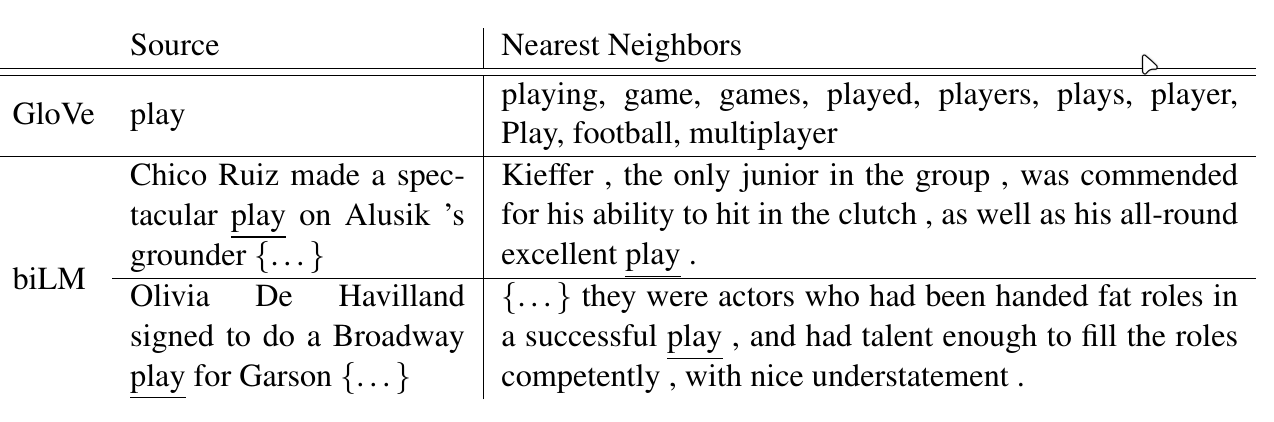
\includegraphics[width=0.85\textwidth]{Sections/3StateOfTheArt/3_images/ELMO.png}
            \caption[Nearest neighbors to "play" using GLoVe]{Nearest neighbors to "play" using GLoVe and context embeddings from a biLM \cite{Peters:2018}.} 
        \end{figure}

        \par GLoVe only uses the word "play" as source, therefore the obtained neighbors for that word are spread across several parts of speech however they all focus on the sports-related sense of the word "play". ELMo biLM uses the entire sentence as source, this means that it is able to understand the context of the word, therefore in both cases, the biLM is able to disambiguate both the part of speech and word sense in the source sentence \cite{Peters:2018}.
        

       
\section{Available NLP libraries}
    \label{sec:libraries}

    There is a wide array of NLP tools and services available. Knowing their features is important in order to find the most appropriate one for the project at hands. Some might be better for smaller project and others better for experts working with big data projects. Furthermore, NLP libraries solve the problem of requiring superior knowledge of mathematics, machine learning, and linguistics. Using these tools, developers can simplify text processing so that they can concentrate on building machine learning models. Some of the libraries created to solve NLP problems will be discussed in the next sections.





        \subsection{SpaCy}
        
        \par SpaCy is a free, open-source library for advanced natural language processing written in Python and Cython published by Explosion AI. It was designed specifically for production use and to help in the building of applications that process and "understand" large volumes of text data.  Some use cases for this specific library are to build information extraction or natural language understanding systems, or to pre-process text for deep learning \cite{Spacy2017}. Some of the features that SpaCy offers are: 

        \begin{itemize}
            \item \textbf{Tokenization} : The segmentation of text into words, punctuation, etc
            \item \textbf{Part-of-Speech Tagging} : The assignment of word types to tokens, like verb, noun, etc
            \item \textbf{Similarity} : The comparison between different words, phrases or text documents and how similar they are.
            \item \textbf{Lemmatization} : The assignment of base forms of words.
        \end{itemize}

      

        \subsection{Natural Language ToolKit}

        \par Developed by Steven Bird, Edward Loper and Ewan Klein in the Department of Computer and Information Science at the University of Pennsylvania, NLTK (Natural Language ToolKit) is a suite of open source program modules, tutorials, problem sets and a leading platform for building Python programs to work with human language data. NLTK covers symbolic and statistical natural language processing, and is interfaced to annotated corpora. This library provides easy-to-use interfaces such as WordNet, along with a suite of text processing libraries for classification, tokenization, stemming, tagging, parsing, and semantic reasoning \cite{Loper2002}. 

        \subsection{Stanford Core NLP}

        \par Developed at Stanford University, Core NLP is library written in Java, however with wrappers for different languages, including Python. This library is fast and some of its components can be integrated to NLTK which boosts efficiency. CoreNLP enables users to derive linguistic annotations for text, including token and sentence boundaries, parts of speech, named entities, numeric and time values, dependency and constituency parses, coreference, sentiment, quote attributions, and relations \cite{Manning2015}.


        \subsection{Gensim}

        \par Gensim ("Generate Similar”) is a Natural Language Processing open-source library for unsupervised topic modeling (a technique to extract the underlying topics from large volumes of text)  and for natural language processing. This python-cython library specializes in finding the semantic similarity between two documents through vector space modeling and topic modeling toolkit. It is capable of building document or word vectors, corpora, performing topic identification, performing document comparison (retrieving semantically similar documents) and analysing plain-text documents for semantic structure. In terms of producing word embedding, gensim allows for the usage of Word2Vec and fastText \cite{rehurek_lrec}.
        
        \subsection{TextBlob}

        TextBlob, also a Python library,  offers an API for performing NLP tasks, like part-of-speech tagging, noun phrase extraction, sentiment analysis, classification, language translation, word inflection, parsing, n-grams, and WordNet integration \cite{textblob}.

        \subsection{Flair}

        Flair allows the usage of state-of-the-art NLP models for entity recognition (NER), part-of-speech tagging (PoS), sense disambiguation and classification \cite{akbik2018coling}.

        \subsection{Polyglot}

        This python NLP package supports various multilingual applications and offers the following tasks
        language detection (196 languages), tokenization (165 languages), named entity recognition (40 Languages), part of speech tagging (16 languages), sentiment analysis (136 Languages) \cite{polyglot:2013:ACL-CoNLL}.
    


        
        \section{Final Remarks}
        \label{sec:final_remarks}

        In this thesis the NLP library that was chosen for the development of the text processing phase of the automatic image retrieval system was SpaCy. This decision was because it offers state-of-the-art NLP models, many useful features, it is easy to use and also because of the simple and well written documentation which makes it very beginner friendly. In addition, there was some prior knowledge thanks to the work developed last year for the ImageCLEF challenge \cite{Ribeiro2019}. 
        
        


\cleardoublepage

\chapter{Initial Work}

\par In this chapter a fundamental tool used was imageAI, which is a Computer Vision Python library that allows developers the ability to easily use state-of-the-art AI features . It supports algorithms for image prediction, custom image prediction, object detection, video detection, video object tracking and image predictions trainings. ImageAI also supports object detection, video detection and object tracking using RetinaNet, YOLOv3 and TinyYOLOv3 trained on COCO dataset. In terms of Machine Learning algorithms imageAI supports 4 trained on the imageNet-1000 dataset. \cite{ImageAI}


\par With the goal of finding the best performing neural network or algorithm for image recognition and for object detection a few test runs were made. These test runs consist on feeding each of the neural networks and algorithms available for image recognition and object detection with one picture manually chosen beforehand. Each neural network and algorithm makes five guesses on what the image represents with a prediction probability that ranges in an interval between [0,100]. This prediction probability represents the certainty of the neural network and algorithm in its guess.
\par In sections \ref{sec:image_test} and \ref{sec:object_test} an overview of three example test runs are presented and analysed.



\section{Image Recognition test runs}
\label{sec:image_test}

\par The imageAI library allows the usage of 4 deep learning neural networks for image recognition which are DenseNet, inceptionV3, ResNet50, and SquezeeNet. The explanation on how these neural networks function is presented in chapter \ref{ch:computervision}. The analysis of the results is in section  \ref{sec:results_image_rec}



    \newpage
    \subsection{Test Run Number 1}

    \par For the first run an image of a dog (breed saluki) was analysed by all 4 neural networks.

    \begin{figure}[htb]
        \centering
        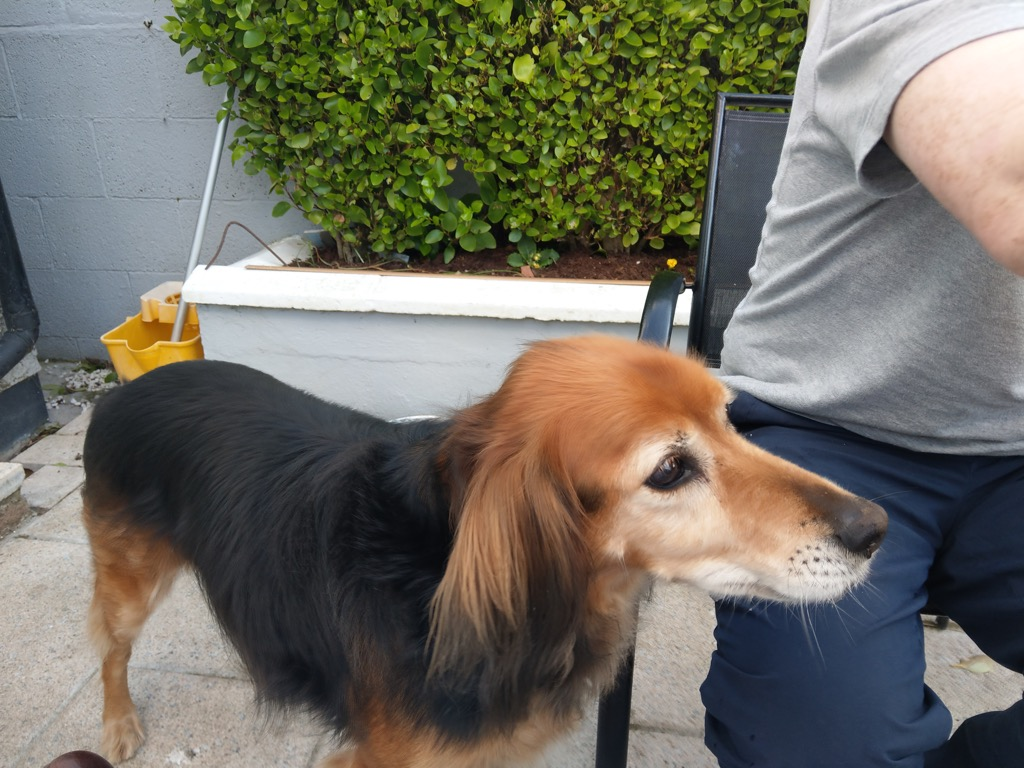
\includegraphics[scale = 0.20]{Sections/4InitialWork/4_images/run1_pic.jpg}
        \caption{First picture to be analysed.} 
    \end{figure}

    \par The obtained results can be seen in the figure below. 

    \begin{figure}[htb]
        \centering
        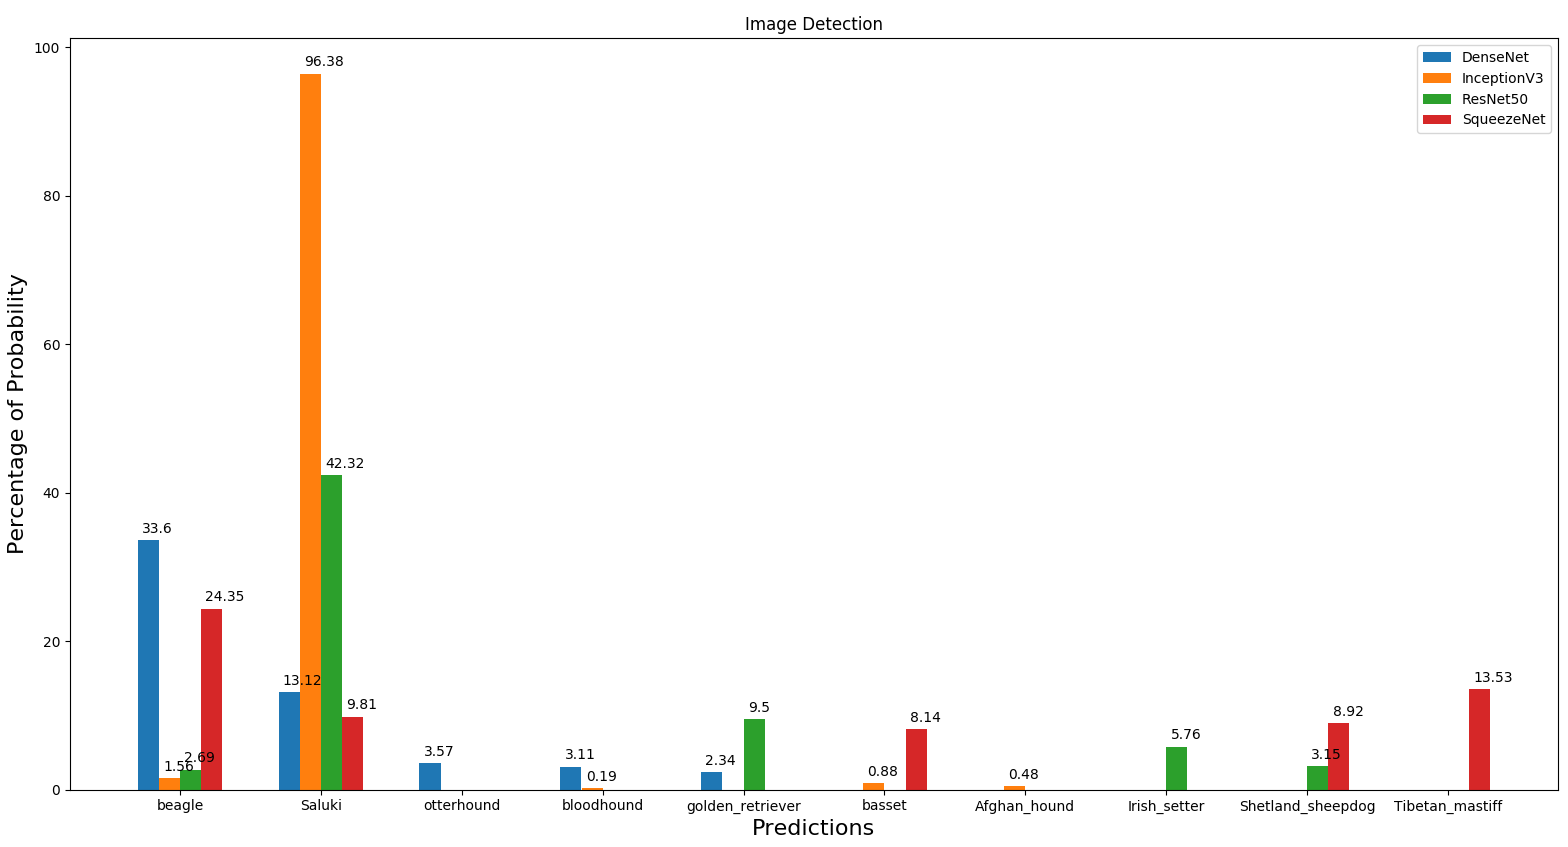
\includegraphics[scale = 0.37]{Sections/4InitialWork/4_images/run1_res.png}
        \caption{Results obtained.} 
    \end{figure}


    \newpage
    \subsection{Test Run Number 2}
    \par For the second run an image of a car was analysed by all 4 neural networks.

    \begin{figure}[htb]
        \centering
        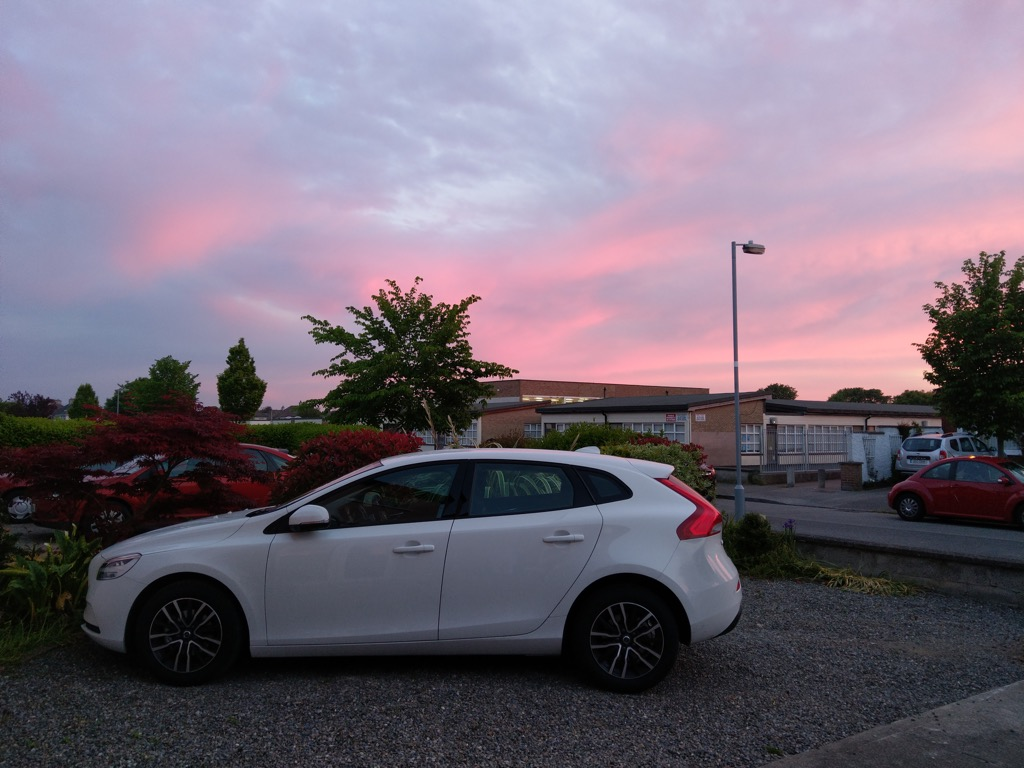
\includegraphics[scale = 0.2]{Sections/4InitialWork/4_images/run3_pic.jpg}
        \caption{Second picture to be analysed.} 
    \end{figure}
    \par The  obtained results can be seen in the image below.
    \begin{figure}[htb]
        \centering
        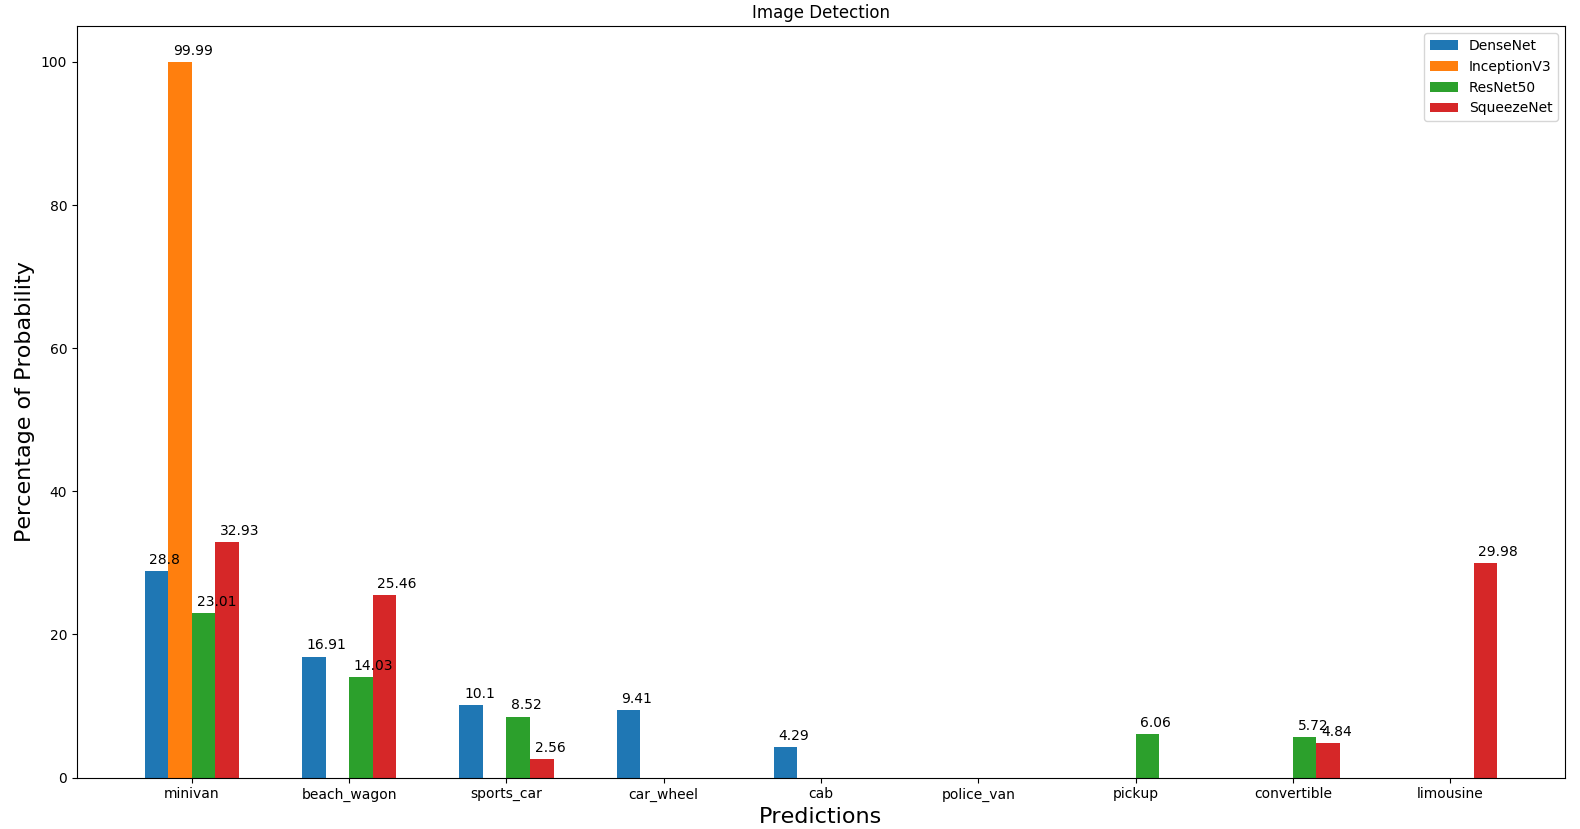
\includegraphics[scale = 0.37]{Sections/4InitialWork/4_images/run3_res.png}
        \caption{Results obtained.} 
    \end{figure}

    \newpage
    \subsection{Test Run Number 3}
    \par For the last run an image of an espresso was analysed by all 4 neural networks.
    \begin{figure}[htb]
        \centering
        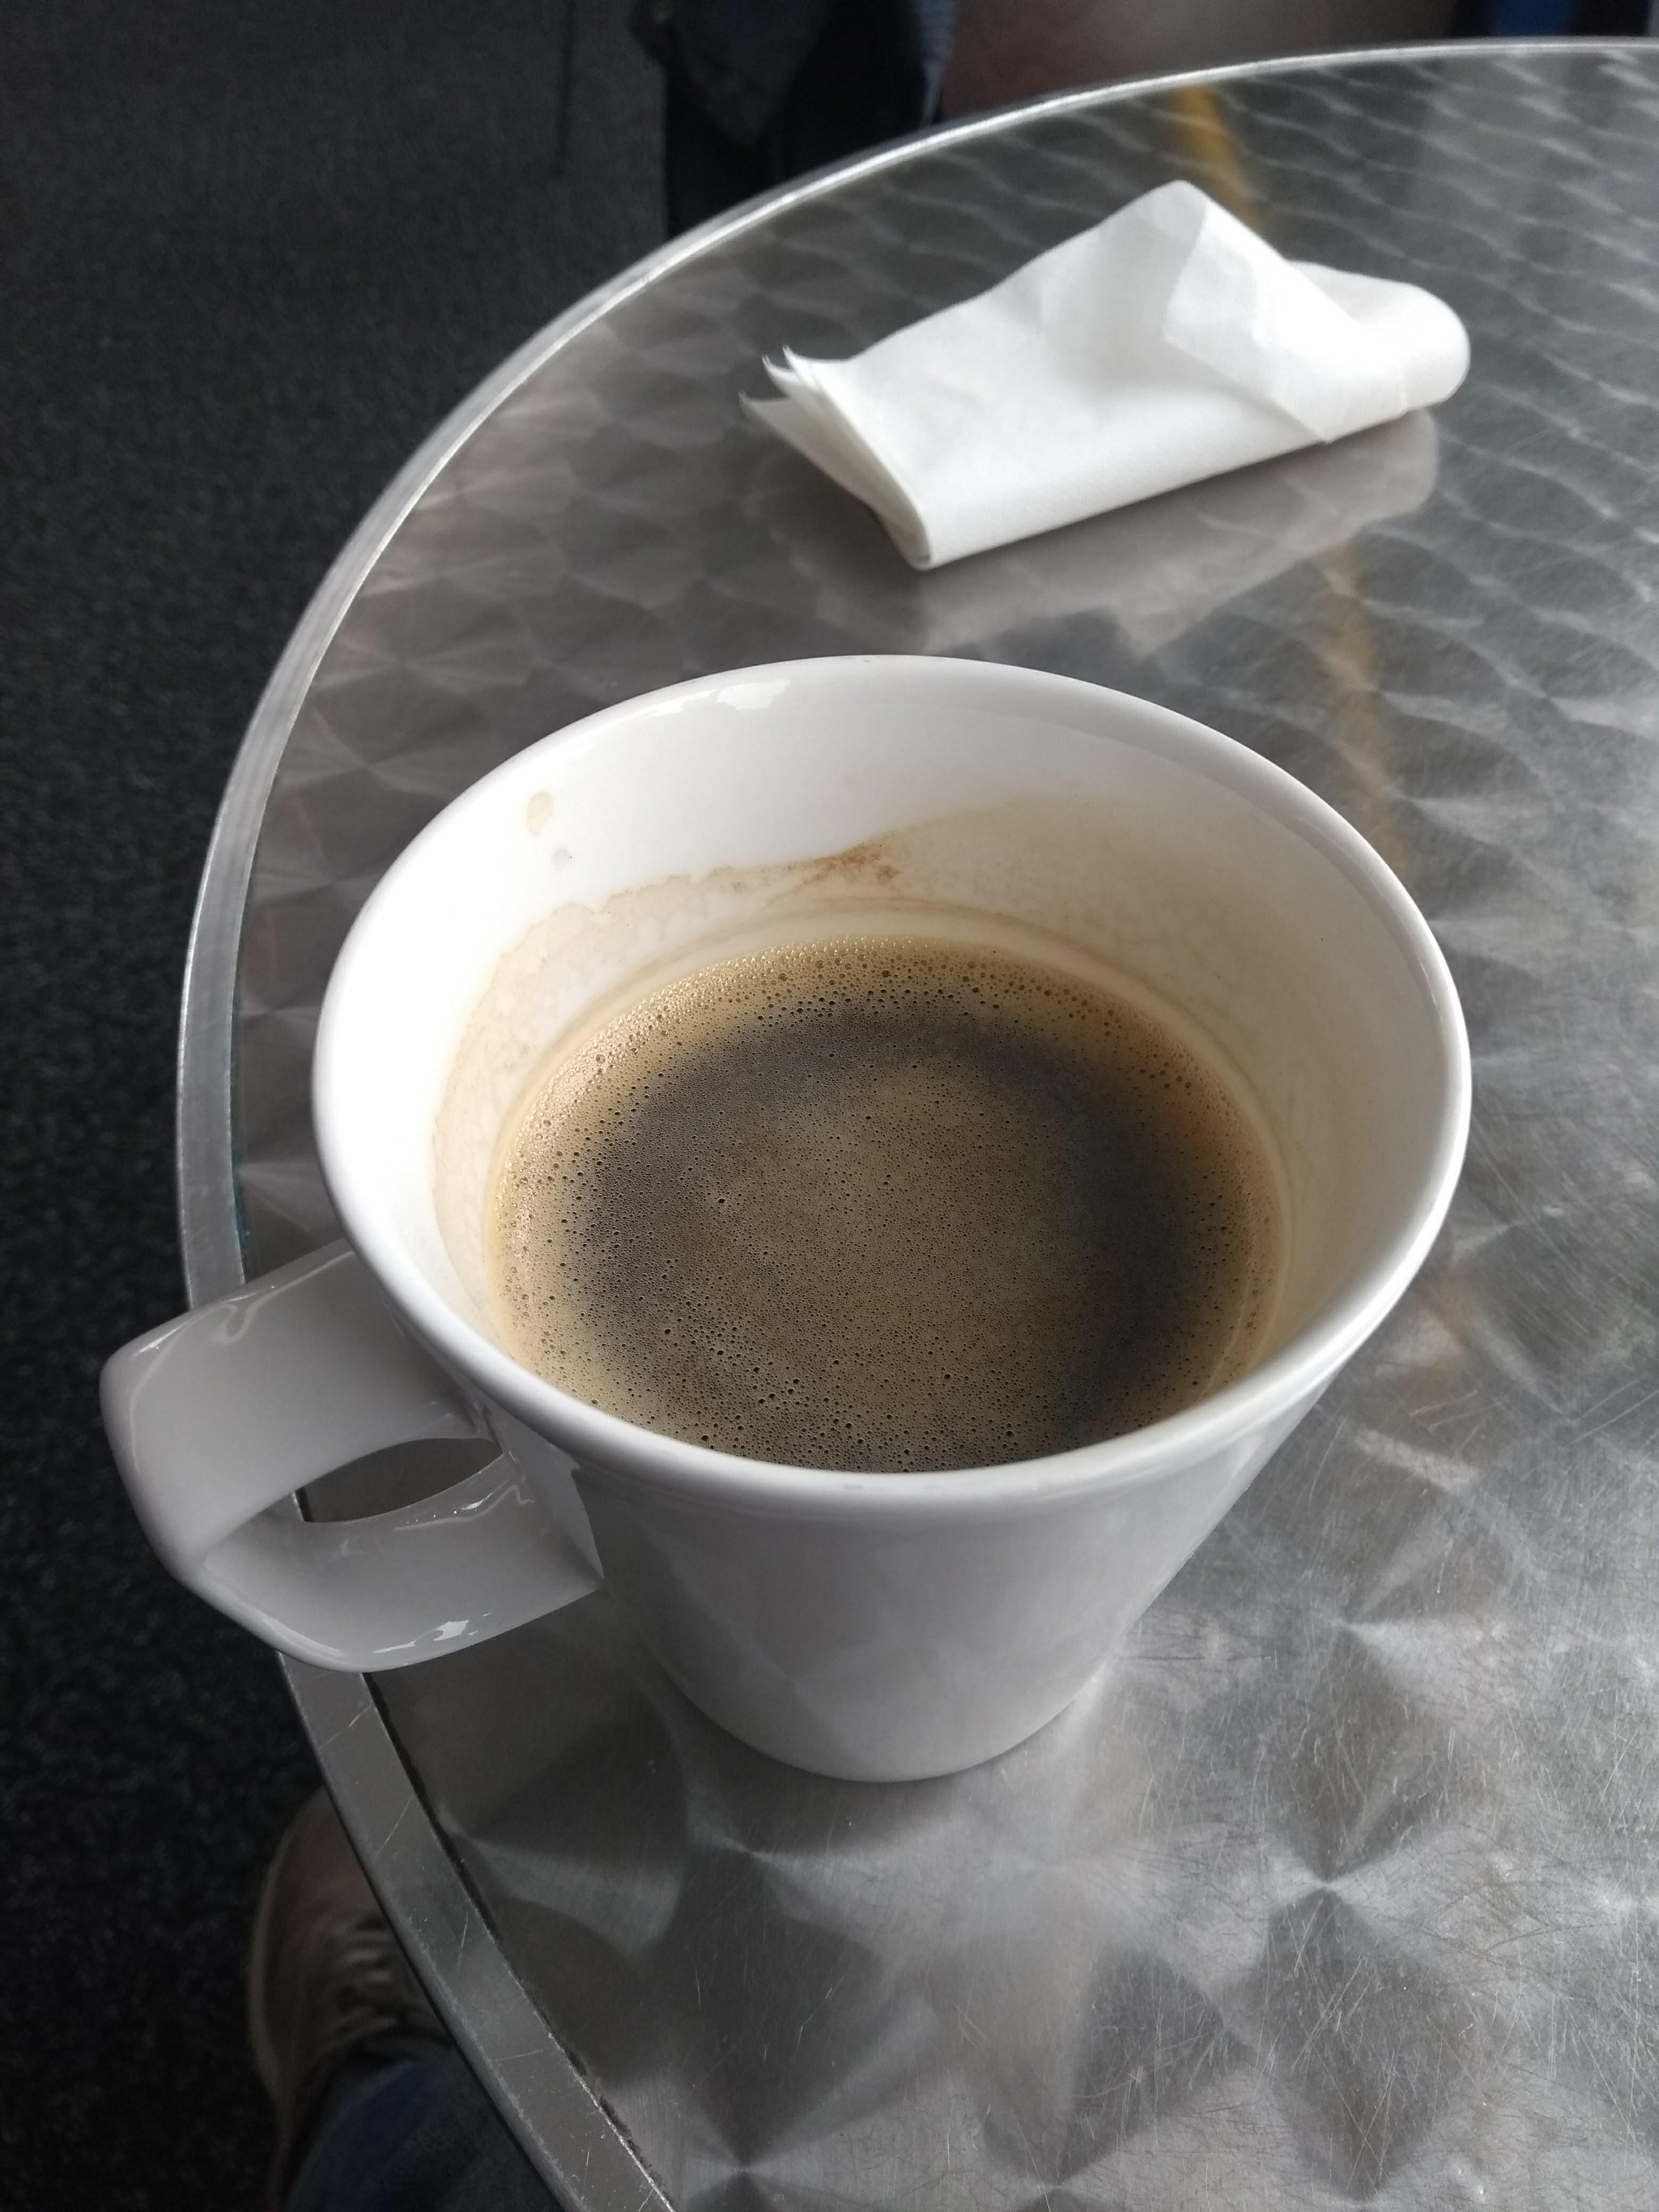
\includegraphics[scale = 0.04]{Sections/4InitialWork/4_images/run4_pic.jpg}
        \caption{Third picture to be analysed.} 
    \end{figure}
    \par The obtained results can be seen in the figure below
    \begin{figure}[htb]
        \centering
        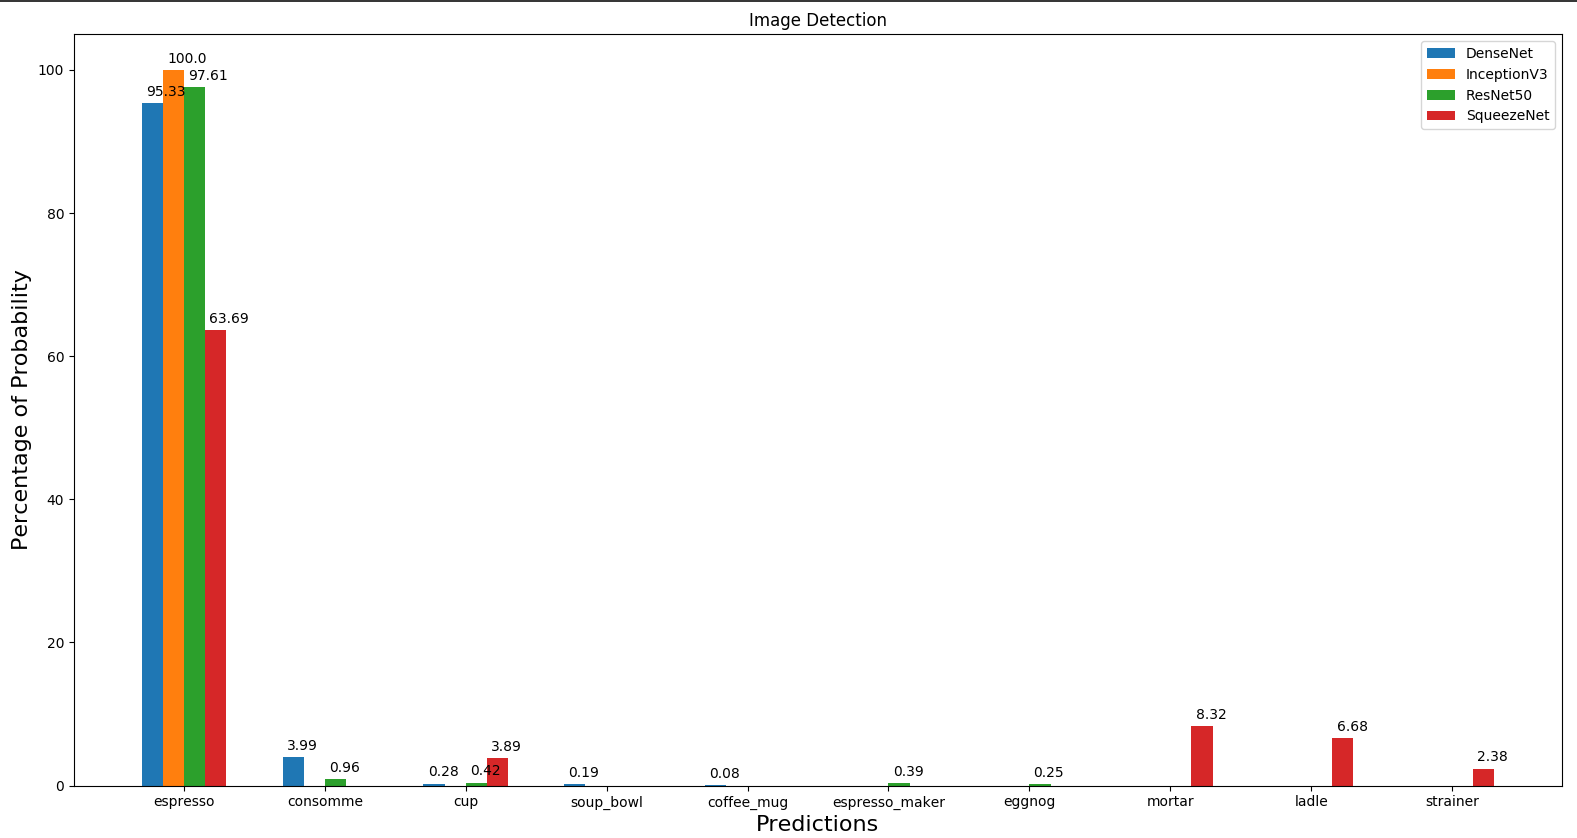
\includegraphics[scale = 0.37]{Sections/4InitialWork/4_images/run4_res.png}
        \caption{Results obtained.} 
    \end{figure}
    
    \newpage
    \subsection{Results analysis}
    \label{sec:results_image_rec}
    



 %%%%%%%%%%%%%%%%%%%%%%%%%%%%%%%%%%%%% OBJECT RECOGNITION   %%%%%%%%%%%%%%%%%%%%%%%%%%%%%%%%%%%%%
\newpage
\section{Object Recognition test runs}
\label{sec:object_test}

\par ImageAI provides 3 different models trained on the COCO dataset for object recognition that are able to identify up to 80 of the most common objects in everyday life. The models provide include RetinaNet, YOLOv3 and TinyYOLOv3. \cite{ImageAI}
\par The explanation on how these algorithms work is presented in chapter \ref{ch:computervision}. The analysis of the results is in section  \ref{sec:results_obj_rec}

    \subsection{Test Run Number 1}

    \begin{figure}[htb]
        \centering
        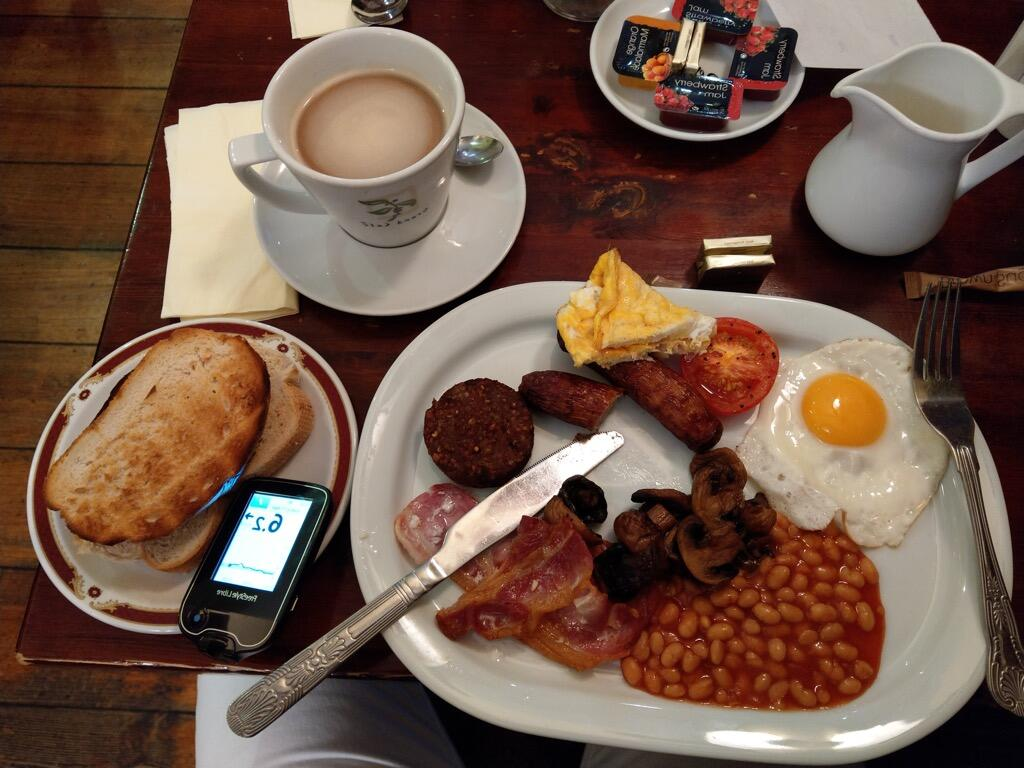
\includegraphics[scale = 0.20]{Sections/4InitialWork/4_images_obj_run1/photo.jpg}
        \caption{First picture to be analysed.} 
    \end{figure}

    \subsubsection{RetinaNet Results}

    \begin{figure}[htb]
        \centering
        \begin{minipage}[b]{0.44\textwidth}
          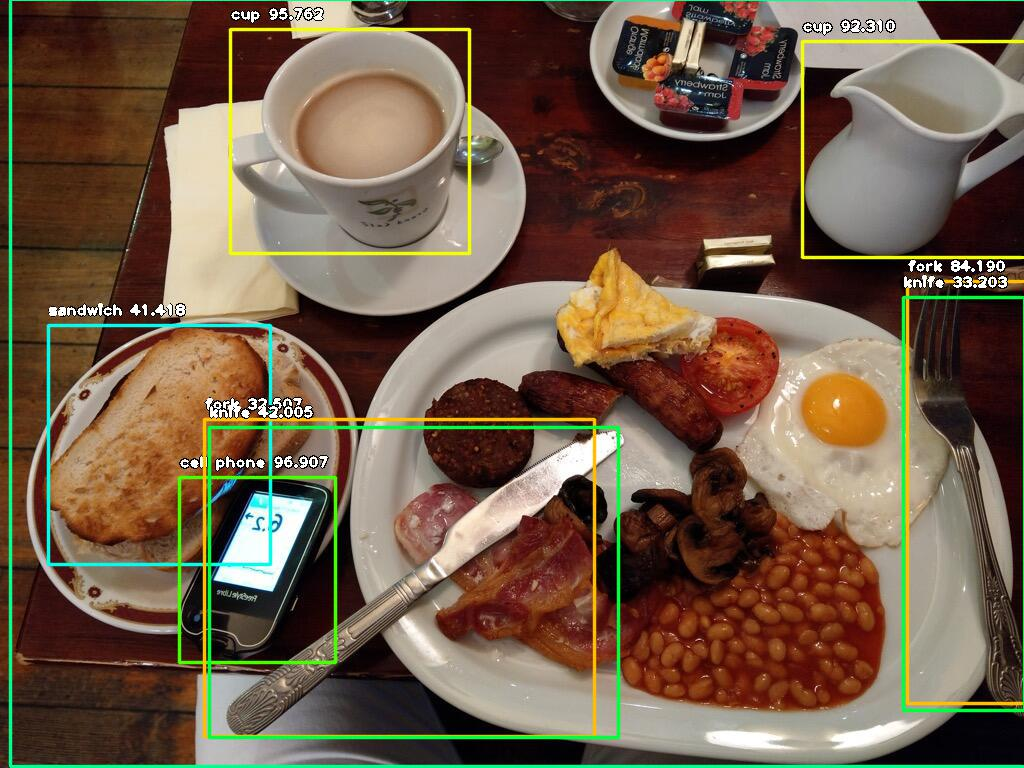
\includegraphics[width=\textwidth]{Sections/4InitialWork/4_images_obj_run1/retinaNet.jpg}
          \caption{RetinaNet Detections.}
        \end{minipage}
        \hfill
        \begin{minipage}[b]{0.50\textwidth}
          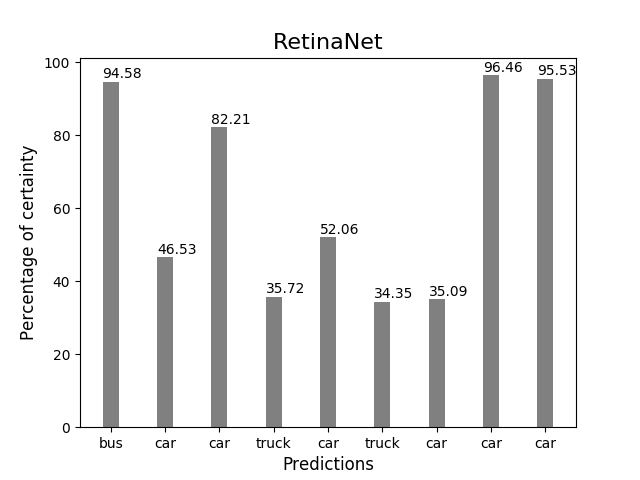
\includegraphics[width=\textwidth]{Sections/4InitialWork/4_images_obj_run1/retinaNet_graph.png}
          \caption{RetinaNet Detections.}
        \end{minipage}
      \end{figure}
    
    \newpage

    \subsubsection{Yolo Results}

    \begin{figure}[htb]
        \centering
        \begin{minipage}[b]{0.44\textwidth}
          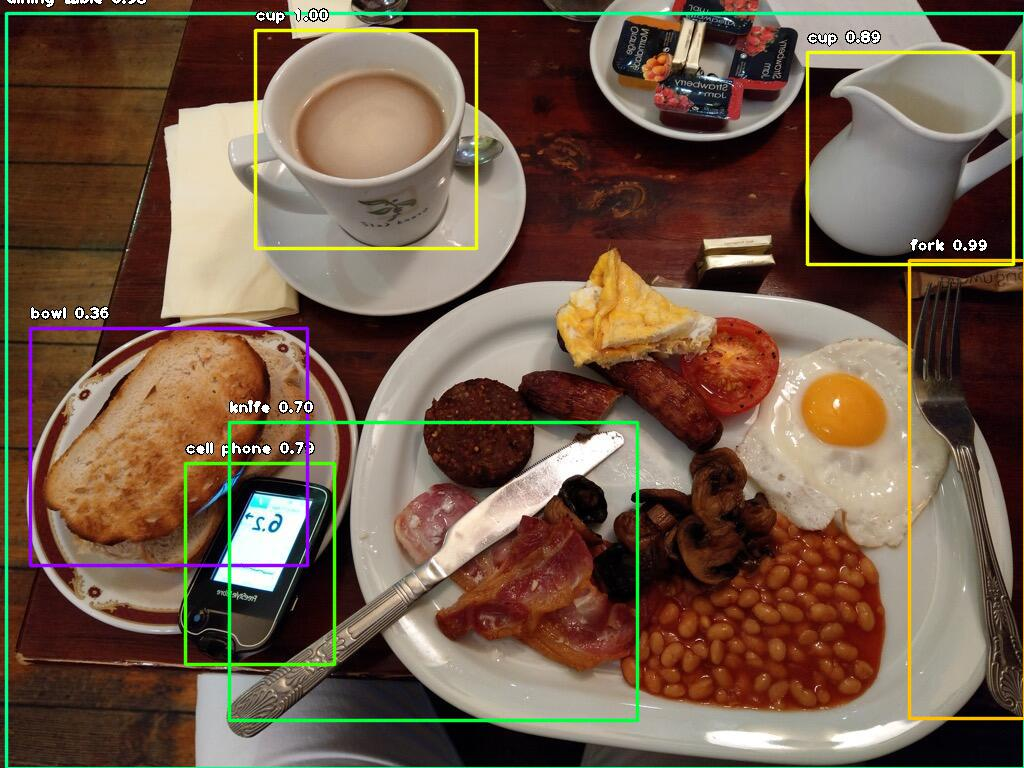
\includegraphics[width=\textwidth]{Sections/4InitialWork/4_images_obj_run1/yolo.jpg}
          \caption{YOLO Detections.}
        \end{minipage}
        \hfill
        \begin{minipage}[b]{0.50\textwidth}
          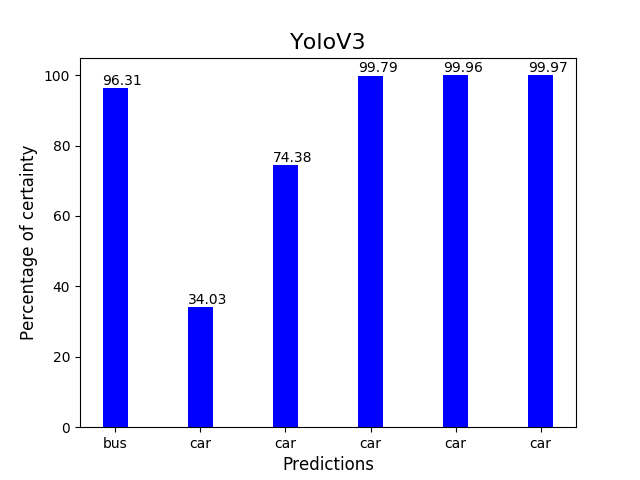
\includegraphics[width=\textwidth]{Sections/4InitialWork/4_images_obj_run1/yolo_graph.png}
          \caption{YOLO Detections.}
        \end{minipage}
      \end{figure}
    
      \subsubsection{TinyYolo Results}

    \begin{figure}[htb]
        \centering
        \begin{minipage}[b]{0.44\textwidth}
          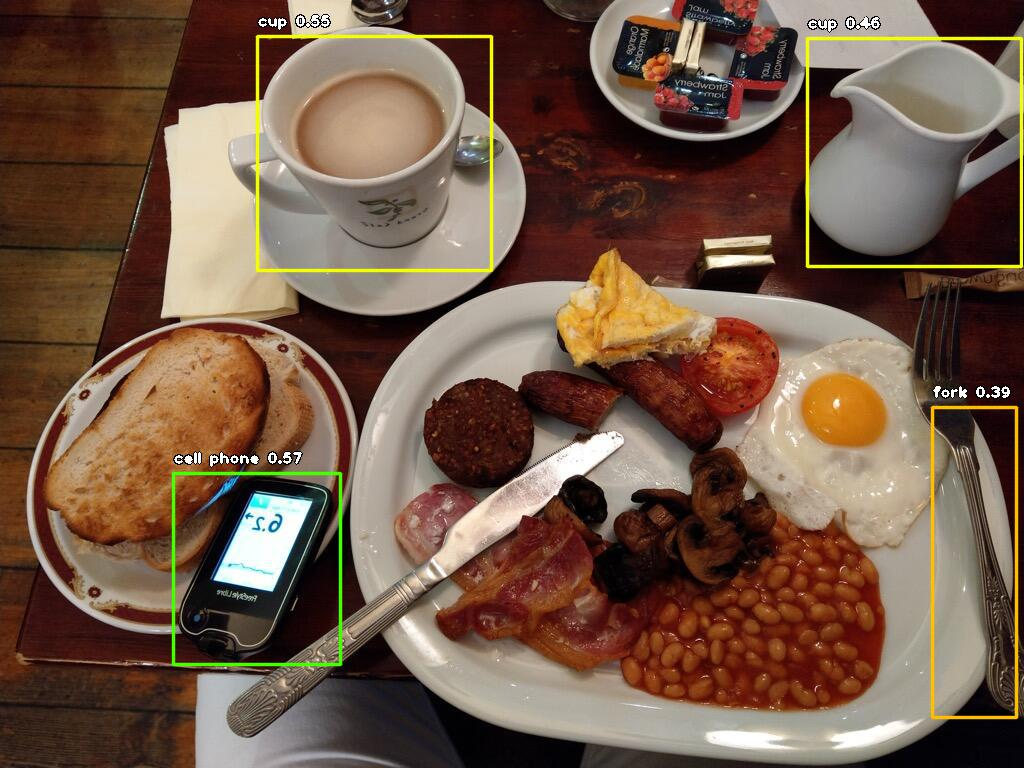
\includegraphics[width=\textwidth]{Sections/4InitialWork/4_images_obj_run1/yolo_tiny.jpg}
          \caption{TinyYolo Detections.}
        \end{minipage}
        \hfill
        \begin{minipage}[b]{0.50\textwidth}
          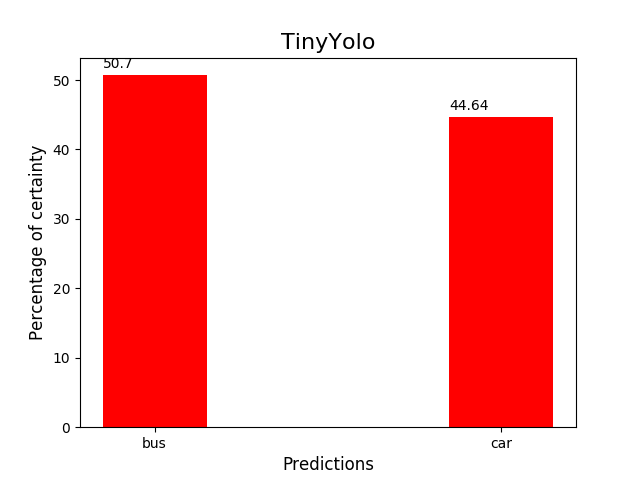
\includegraphics[width=\textwidth]{Sections/4InitialWork/4_images_obj_run1/yolo_tiny_graph.png}
          \caption{TinyYolo Detections.}
        \end{minipage}
      \end{figure}

    \newpage

 %%%%%%%%%%%%%%%%%%%%%%%%%%%%%%%%%%%%% run2   %%%%%%%%%%%%%%%%%%%%%%%%%%%%%%%%%%%%%
    \subsection{Test Run Number 2}

    \begin{figure}[htb]
        \centering
        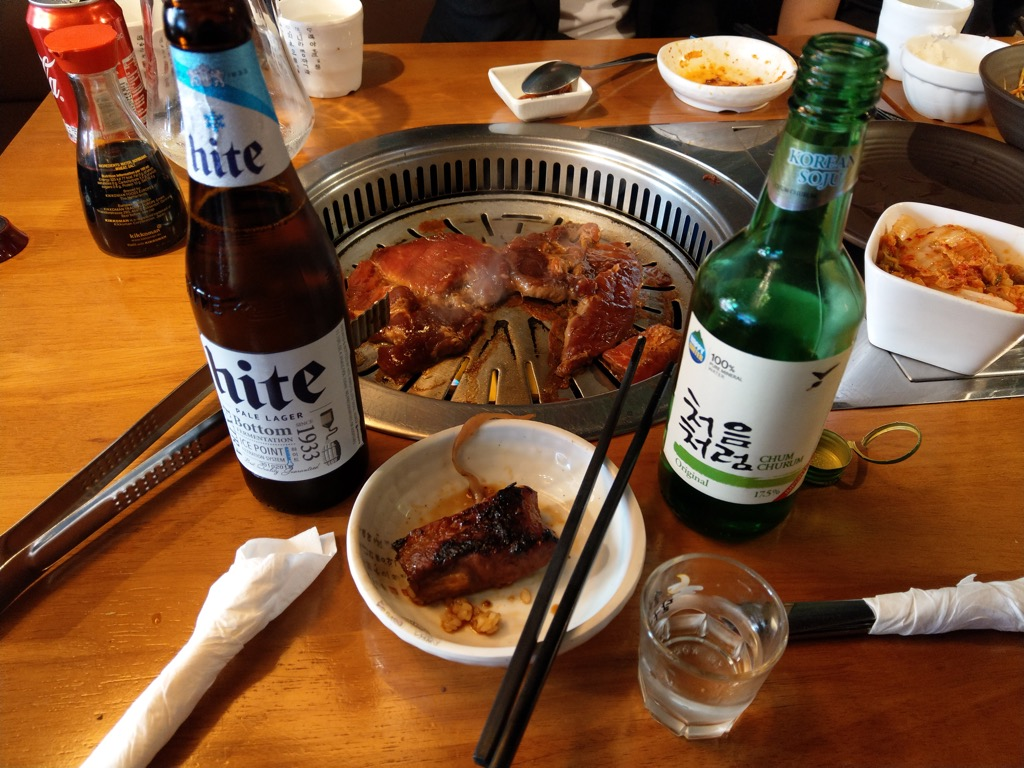
\includegraphics[scale = 0.20]{Sections/4InitialWork/4_images_obj_run2/photo.jpg}
        \caption{Second picture to be analysed.} 
    \end{figure}

    \subsubsection{RetinaNet run 2 results}

    \begin{figure}[htb]
        \centering
        \begin{minipage}[b]{0.44\textwidth}
          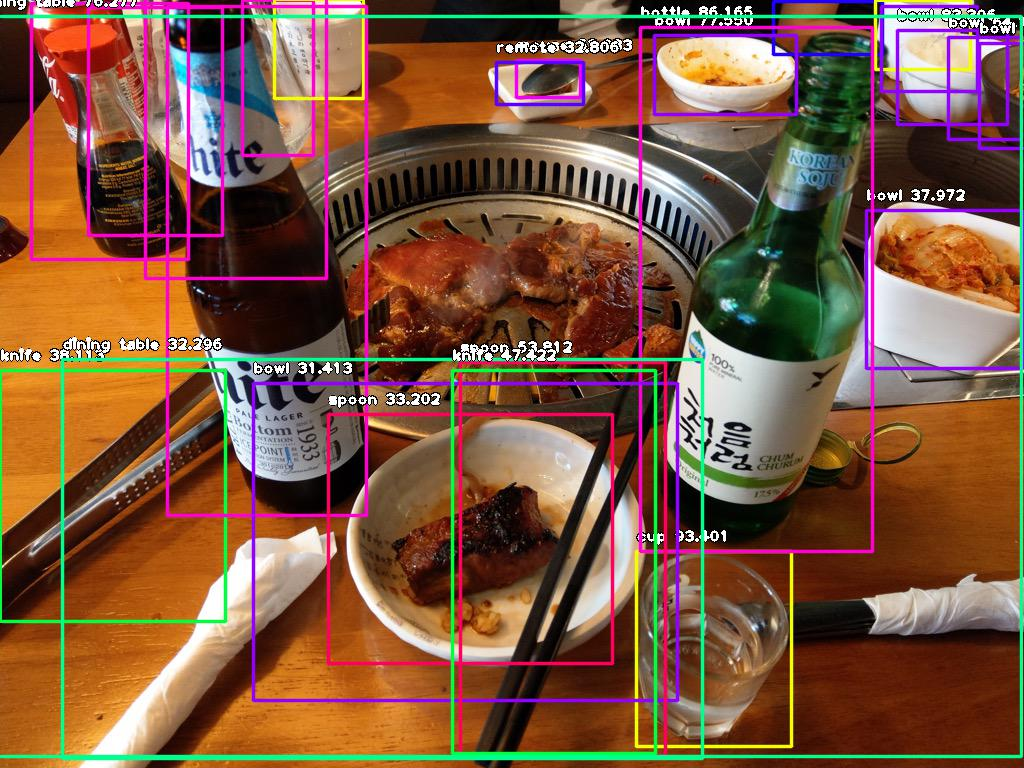
\includegraphics[width=\textwidth]{Sections/4InitialWork/4_images_obj_run2/retinaNet.jpg}
          \caption{RetinaNet Detections.}
        \end{minipage}
        \hfill
        \begin{minipage}[b]{0.50\textwidth}
          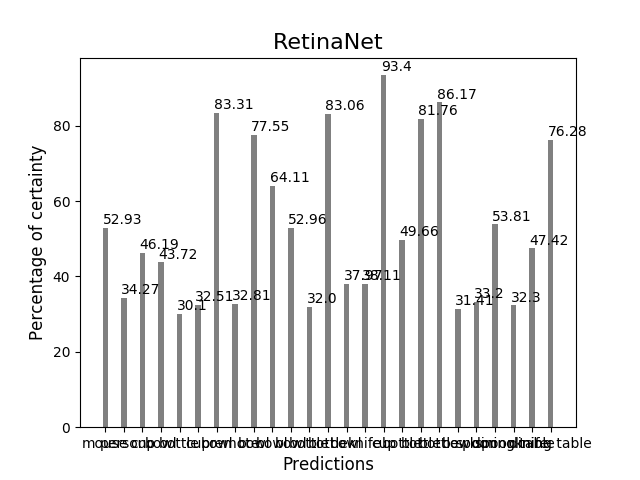
\includegraphics[width=\textwidth]{Sections/4InitialWork/4_images_obj_run2/retinaNet_graph.png}
          \caption{RetinaNet Detections.}
        \end{minipage}
      \end{figure}
    
    \newpage

    \subsubsection{Yolo run 2 results}

    \begin{figure}[htb]
        \centering
        \begin{minipage}[b]{0.44\textwidth}
          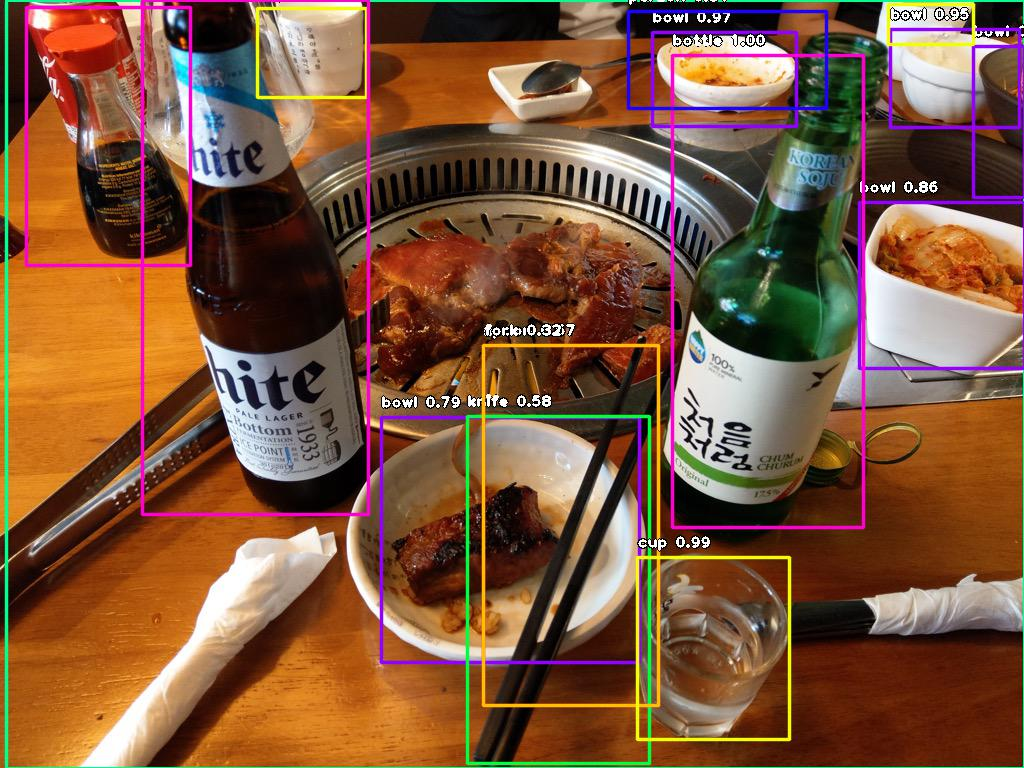
\includegraphics[width=\textwidth]{Sections/4InitialWork/4_images_obj_run2/yolo.jpg}
          \caption{YOLO Detections.}
        \end{minipage}
        \hfill
        \begin{minipage}[b]{0.50\textwidth}
          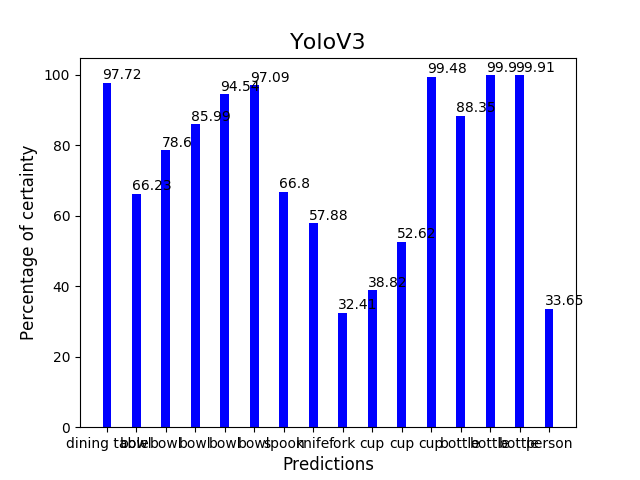
\includegraphics[width=\textwidth]{Sections/4InitialWork/4_images_obj_run2/yolo_graph.png}
          \caption{YOLO Detections.}
        \end{minipage}
      \end{figure}
    
      \subsubsection{TinyYolo run 2 results}

    \begin{figure}[htb]
        \centering
        \begin{minipage}[b]{0.44\textwidth}
          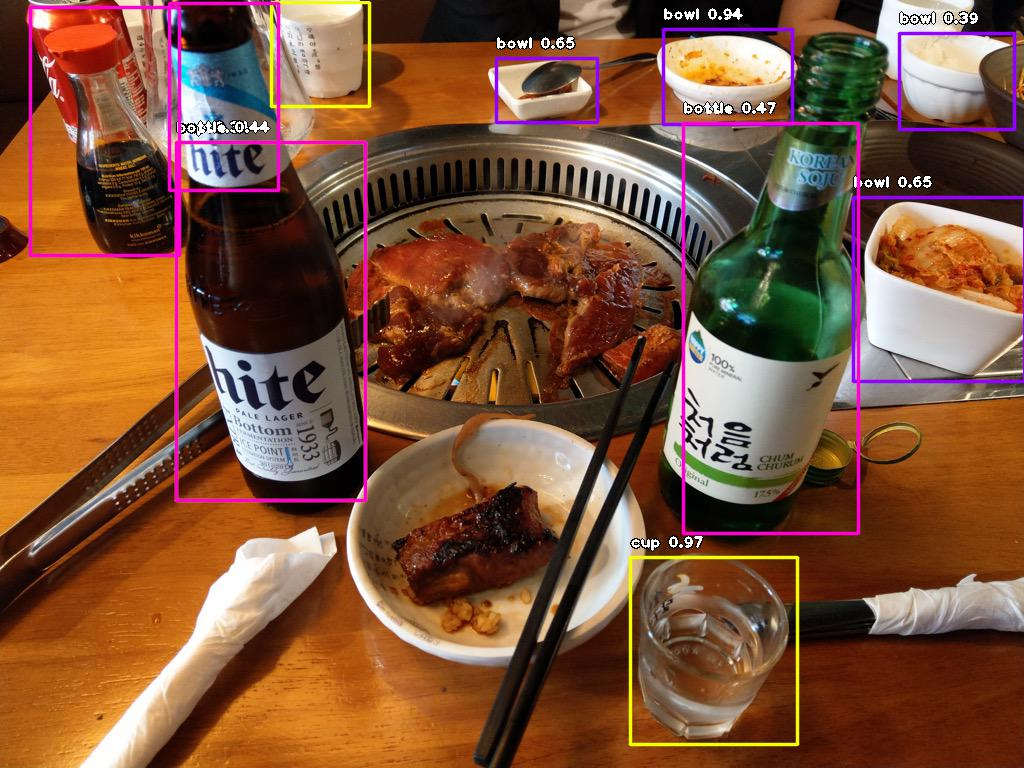
\includegraphics[width=\textwidth]{Sections/4InitialWork/4_images_obj_run2/yolo_tiny.jpg}
          \caption{TinyYolo Detections.}
        \end{minipage}
        \hfill
        \begin{minipage}[b]{0.50\textwidth}
          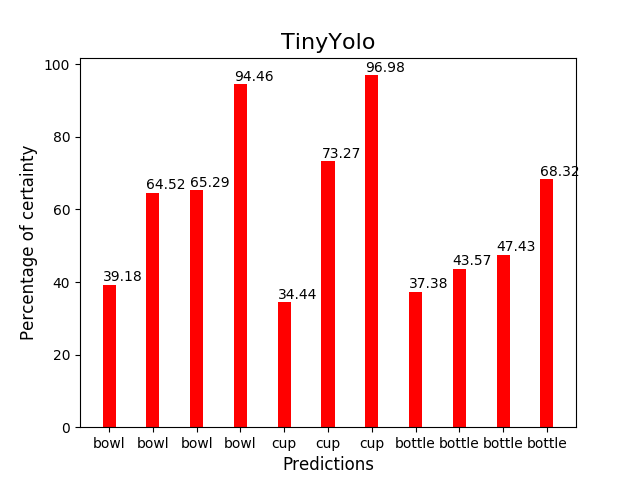
\includegraphics[width=\textwidth]{Sections/4InitialWork/4_images_obj_run2/yolo_tiny_graph.png}
          \caption{TinyYolo Detections.}
        \end{minipage}
      \end{figure}

    \newpage


 %%%%%%%%%%%%%%%%%%%%%%%%%%%%%%%%%%%%% run3 %%%%%%%%%%%%%%%%%%%%%%%%%%%%%%%%%%%%%
    \subsection{Test Run Number 3}

    \begin{figure}[htb]
        \centering
        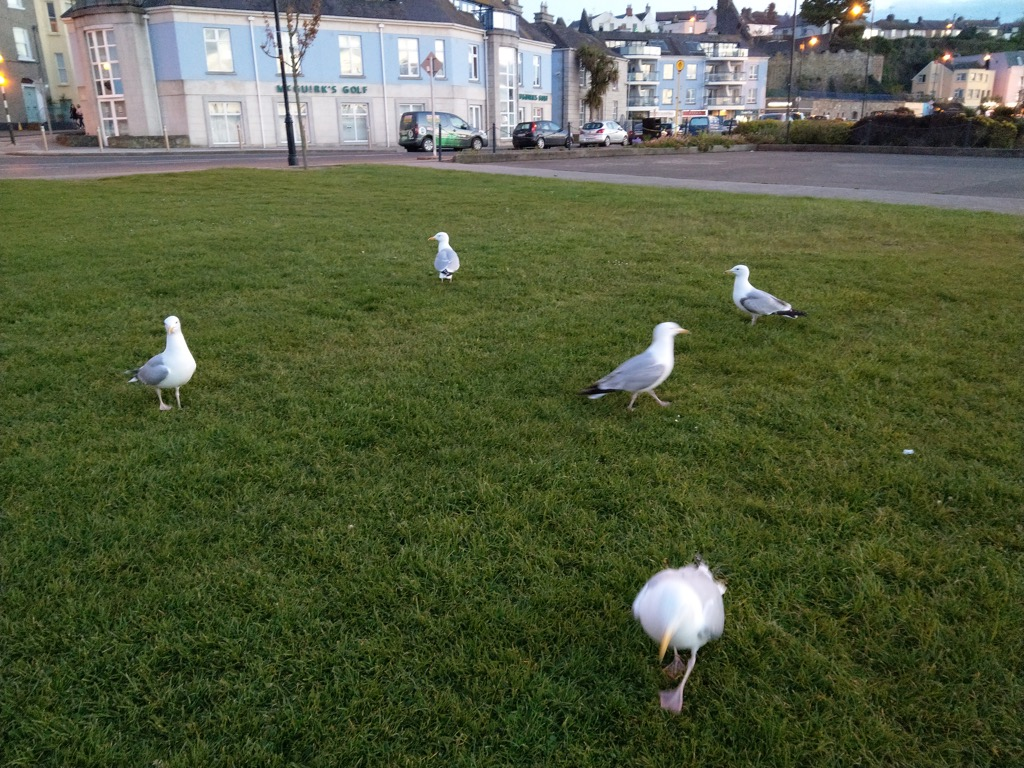
\includegraphics[scale = 0.20]{Sections/4InitialWork/4_images_obj_run3/photo.jpg}
        \caption{Third picture to be analysed.} 
    \end{figure}

    \subsubsection{RetinaNet Results}

    \begin{figure}[htb]
        \centering
        \begin{minipage}[b]{0.44\textwidth}
          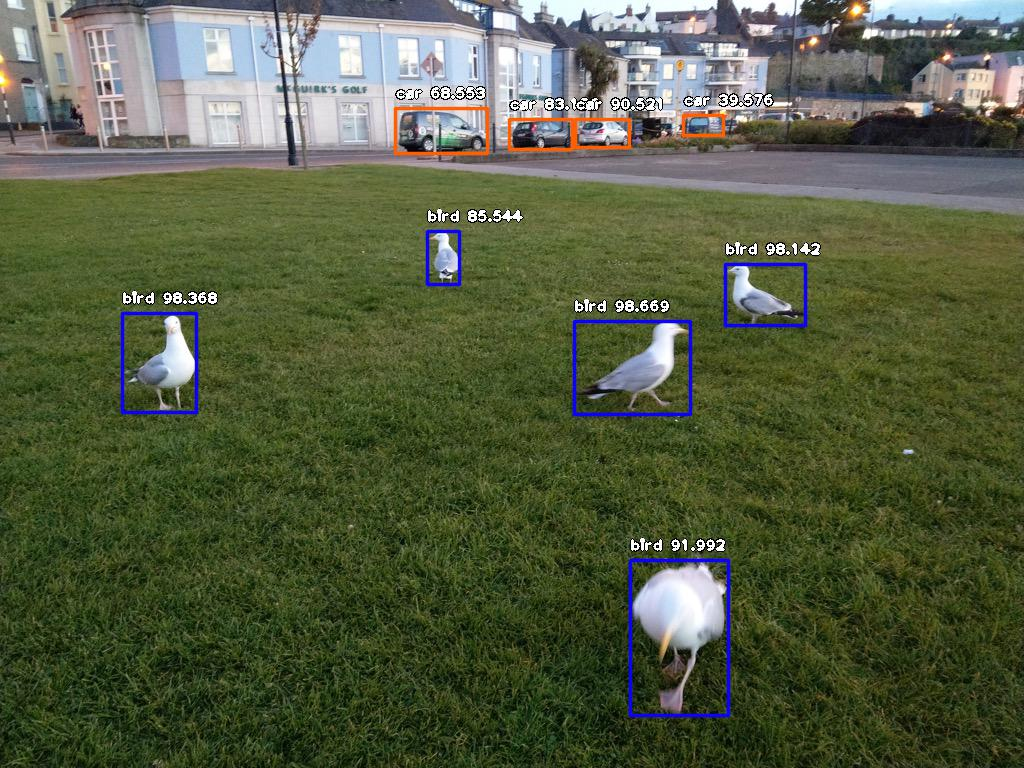
\includegraphics[width=\textwidth]{Sections/4InitialWork/4_images_obj_run3/retinaNet.jpg}
          \caption{RetinaNet Detections.}
        \end{minipage}
        \hfill
        \begin{minipage}[b]{0.50\textwidth}
          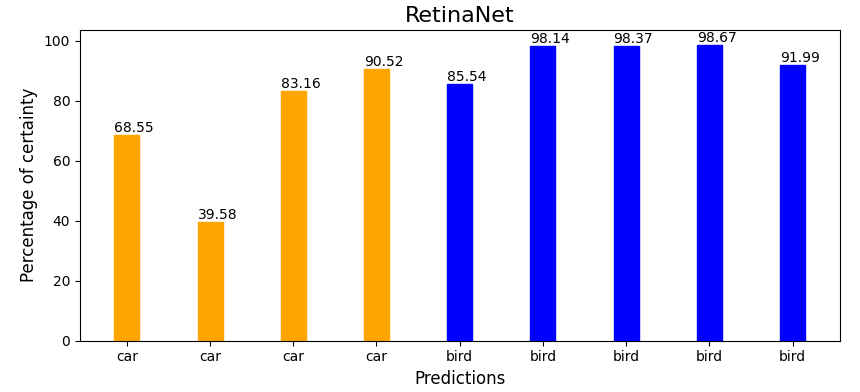
\includegraphics[width=\textwidth]{Sections/4InitialWork/4_images_obj_run3/retinaNet_graph.png}
          \caption{RetinaNet Detections.}
        \end{minipage}
      \end{figure}
    
    \newpage

    \subsubsection{YOLO Results}
    
    \begin{figure}[htb]
        \centering
        \begin{minipage}[b]{0.44\textwidth}
          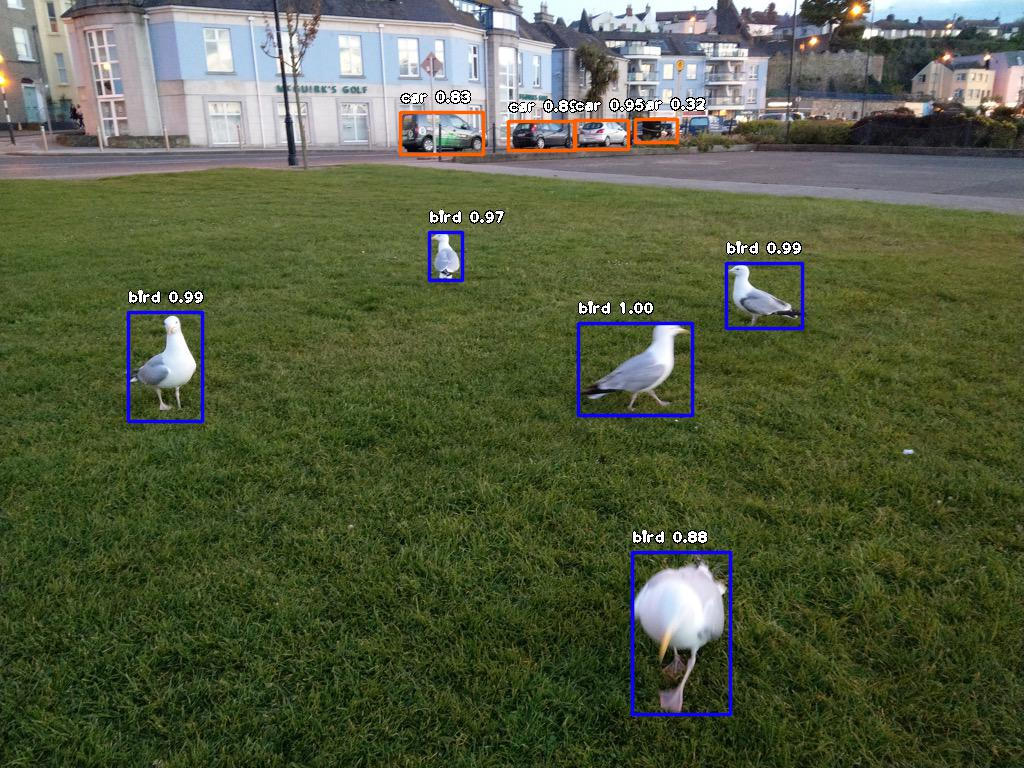
\includegraphics[width=\textwidth]{Sections/4InitialWork/4_images_obj_run3/yolo.jpg}
          \caption{YOLO Detections.}
        \end{minipage}
        \hfill
        \begin{minipage}[b]{0.50\textwidth}
          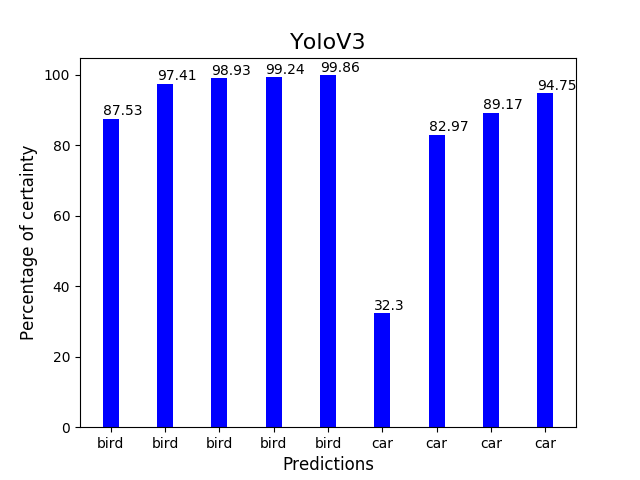
\includegraphics[width=\textwidth]{Sections/4InitialWork/4_images_obj_run3/yolo_graph.png}
          \caption{YOLO Detections.}
        \end{minipage}
      \end{figure}
    
      \subsubsection{TinyYOLO Results}

    \begin{figure}[htb]
        \centering
        \begin{minipage}[b]{0.44\textwidth}
          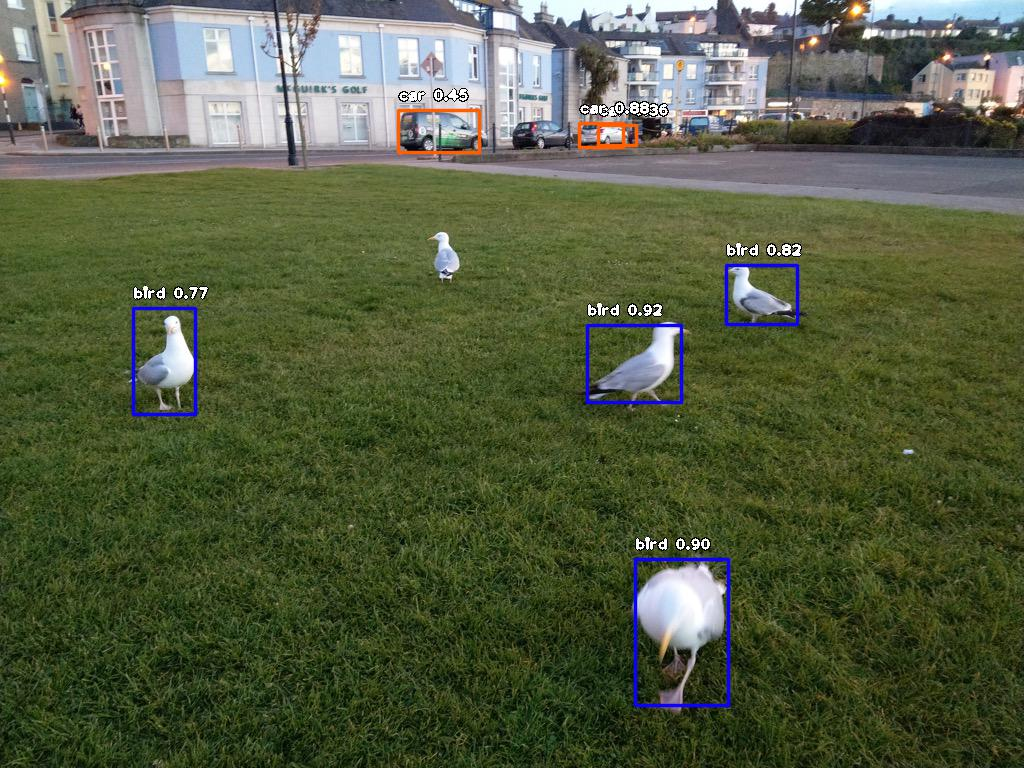
\includegraphics[width=\textwidth]{Sections/4InitialWork/4_images_obj_run3/yolo_tiny.jpg}
          \caption{TinyYolo Detections.}
        \end{minipage}
        \hfill
        \begin{minipage}[b]{0.50\textwidth}
          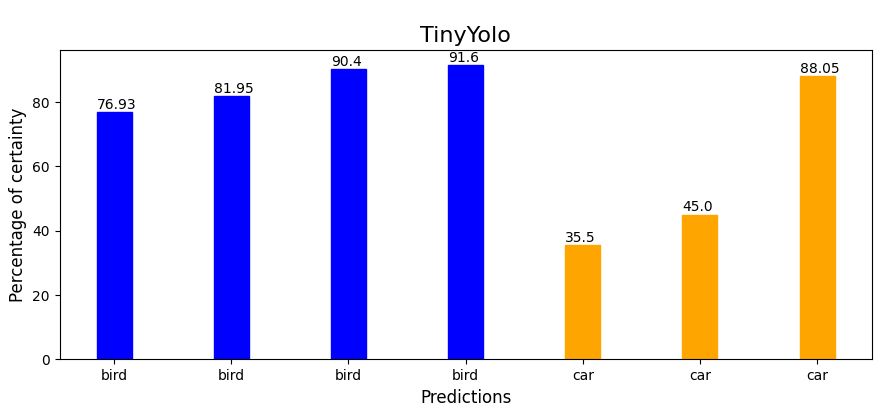
\includegraphics[width=\textwidth]{Sections/4InitialWork/4_images_obj_run3/yolo_tiny_graph.png}
          \caption{TinyYolo Detections.}
        \end{minipage}
      \end{figure}

    \newpage
    \subsection{Results analysis}

    \label{sec:results_obj_rec}


\chapter{The Automatic Retrieval system}

This chapter aims at explaining how the text processing system was created and how it manages to extract relevant information from text like activities, locations, objects and so on.



\section{Text Processing and Word Extraction}

In the text processing stage, the query topics are analysed using Natural Language Processing tools to extract relevant words in order to retrieve the desired moment. Those words are compared with the visual concepts words obtained in the image processing stage. The text is therefore processed using a pre-trained state-of-the-art word2vec model in order to produce word embeddings.

The SpaCy library is used to analyse the query topics fully, extracting relevant words from the title, the description and narrative. The words extracted are divided into 10 categories being them : "relevant things", "activities", "dates", "locations", "inside", "outside", "negative relevant things", "negative activities", "negative locations" and "negative dates".

In order to assign words to each category some linguistic rules were defined,
such as semantic and syntactic rules. Semantic rules build the meaning of the
sentence from its words and how words combine syntactically. Syntax rules refer to
the rules that govern the ways in which words combine to form phrases, and
sentences. 

\begin{figure}[H]
    \centering
    \captionsetup{justification=centering}
    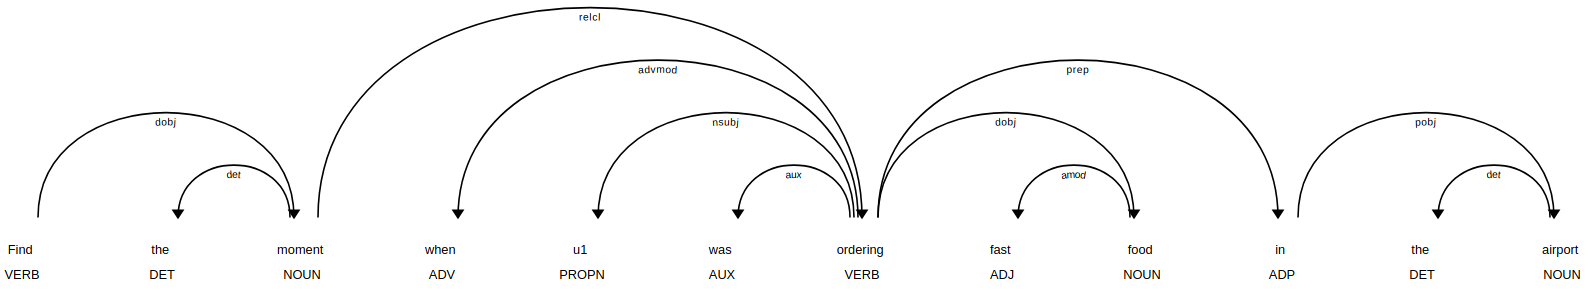
\includegraphics[width = 0.9 \textwidth]{Sections/6textprocessing/images/spacy.png}
    \caption{Linguistic annotations generated by SpaCy library for the narrative of the topic 6 of the test topics.}
    \label{fig:spacy_labels}
  \end{figure}
  
  
  
  As an example, some of the rules that were applied in the extraction of words to different categories:
  
  \begin{itemize}
      \item  If the word is a "VERB" and ends with "ing", like "ordering" then it probably is an activity and if the words that follows are "NOUN" with or without "ADJ" (adjectives) then those words are probably either a location or an object.
      \item  If the word is and "ADP" and its either "in" or "at" then the words that follow are probably locations and usually means that the moment occurs inside a location and not outside, the category "inside" is then flagged to "True" and "outside" is flagged to "False".
      \item If the word is a "NUM" (number) then it probably refers to a year.
      \item if the sentence has an auxiliary verb, the main verb usually corresponds to an activity and the words that follow the main verb may be objects or locations.
      \item If the word is an "ADJ" (adjective) then the following word is probably an object. It can also be a bi-gram like "ice cream" or in this case "fast food".
      \item If the sentence ends with "not considered relevant" the extracted words go to the negative categories.
      \item Rules for the extraction of dates, like day of the week, months, years, were also created, but do the the syntax of the test topics they were discarded in order to save time, however, for the dev topics they were used and produced good results. As an example if in the topic it was said that the moment happened on a "wednesday" or in year 2014, only pictures from wednesday or the year 2014 were retrieved.

    \end{itemize}


Using figure \ref{fig:spacy_labels} as an example, the extracted words for the different categories for the topic narrative of topic 6 from the test topics were as follows:

    \begin{itemize}
        \item \textbf{relevant things} : "fast food".
        \item \textbf{activities} : "ordering", "ordering fast food".
        \item \textbf{locations} : "airport".
        \item \textbf{inside} : "True".
        \item \textbf{outside}: "False".
       
    \end{itemize}


\section{Retrieval}

    In the retrieval step the images are recovered according to the desired query topic.
    As an example figure \ref{fig:testtopic} represents the test topic number 7.
   
    \begin{figure}[H]
        \centering
        \captionsetup{justification=centering}
        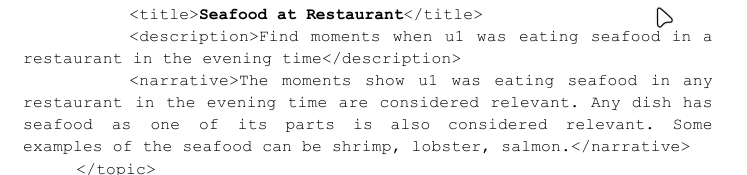
\includegraphics[width = \textwidth]{Sections/6textprocessing/images/topic.png}
        \caption{Test topic number 7.}
        \label{fig:testtopic}
      \end{figure}
      
      The extracted words of the title, description and narrative are as follows:

      \begin{itemize}
        \item \textbf{relevant things} : 
            "seafood",
            "parts",
            "shrimp",
            "lobster",
            "salmon".
        \item \textbf{activities} : "eating",
        "eating seafood"
        \item \textbf{locations} : "restaurant",  "evening time".
        \item \textbf{inside} : "True".
        \item \textbf{outside}: "False".
        \item \textbf{dates}: NULL.
        \item \textbf{negative relevant thing}: NULL.
        \item \textbf{negative activities}: NULL.
        \item \textbf{negative locations}:  NULL.
        \item \textbf{negative dates}: NULL.
       
    \end{itemize}

    The words "evening time" went to the locations category wrongly because of the previously described rule, where if a word is an "ADP" and it is "in" then the following "NOUN" is probably a location, which in this case is not correct.


    A comparison is made between the visual concept words extracted from the images and the words extracted from the topic. In order to do this, the SpaCy en\_core\_web\_md model was used, which is an english mult-task CNN trained on OntoNotes, with GloVe vectors trained on Common Crawl. This model allows for the computation of the similarity between words.

    For example the word "television" and "seafood" have a similarity of 0.0705759162558067 while "television" and "screen" have a similarity of 0.4271196001925812.

    Afterwards, a confidence score is computed for each image in the dataset for every single topic, which means that a confidence score was calculated for 2.000.000 images, which took a lot of computer processing time and resources, and made it extremely difficult to make adjustments and correct errors.

    The score is obtained through the comparison of the extracted words from the
    topic and the extracted labels from the images. The 10 pictures with the highest confidence score for each topic are retrieved.

    \section{Run 1 and Run 2 }
    Using figure \ref{fig:image_fully_processed}, the comparisons made are the following :

    \begin{itemize}
        \item The category "concepts" is compared to the category "relevant things";
        \item The category "activity" is compared to the category "activities";
        \item The category "location" is compared to the category "locations";
        \item "Depending if "inside" = "True" / "False" the "io\_score" value will have different impact.
        \item Do to the fact that the labels extracted from the Places model are sometimes not accurate enough and that the textual data extracted from the topic is not specific enough, the category "categories" and "attributes" was discarded from counting to the confidence score in order to save time.
    \end{itemize}
    

 This confidence score is influenced by the
scores of the image concepts obtained through the object detection phase and
the different weights assigned to each category. The weight for each category is
obtained through two different factors, a factor of importance and a computed
factor.

In Run 1, the importance factor for all categories is the same. This means
that each category has the same weight for the computation of the confidence
score.

For Run 2, it was decided to define the importance factor differently for each category. It was given a bigger importance to specific categories like "relevant things" in order to improve results, since the computation of the similarity of this textual category with the extracted object detection image label concepts. Categories like
”activities” and ”locations” get a lesser importance factor since they are being
compared to the organizers label data which is limiting and lesser accurate. The
sum of all importance factors of all categories is equal to 1, which represents
100\%.

The computed factor is obtained from the distribution of the factor of importance from empty categories to all other categories. If there isn't any
textual data extracted from a query topic for the category ”activities”, this category will
be empty, therefore, the  the importance factor of the ”activities” is apportioned
 to all other categories, increasing their importance factor, in order to
maintain the sum of 1.

This value is not the same for each category, the ratio of the distribution is equal to the default ratio of the importance factor of all categories. To make it clearly, if the importance factor for ”relevant things” is 0.5, which is half of the sum of all importance factors, and
if the ”activities” category is worth 0.2 and has no extracted textual data, then
half of 0.2 is distributed to ”relevant things”, which increases the importance to
0.6 and the remainder 0.1 will be distributed the same way to other categories
ensuring that the sum of all importance factors is 1.

The negative categories works the same way, but instead of contributing for
the confidence score, it decreases the value of the confidence.

A general threshold was previously defined in order to remove images of low
concept scores or low confidence score, images above the threshold are selected
for the query topic. The threshold was implemented through some trial and
error during the test phases, and it merely serves the purpose of saving some
computational time.

Run 2 differs from Run 1 not only in the image processing step, where differ-
ent image processing algorithms were used, but also in the retrieval step, where
all factors of importance were altered in order to give more importance to some
categories than others, as previously discussed. Another difference is the nega-
tive category which was discarded from the calculation of the confidence score
in Run 2.

Finally, a script runs through all the selected confidence scores for a given
query topic and stores the fifty highest on the csv file. As expected by the
previous year results, this automatic and exhaustive approach is not the most
suitable for a lifelog application.




%%%%%%%%%%%%%%%%%%%%%%%%%%%%%%%%%%%%%
% Bibliografia
\cleardoublepage
\nocite{*}
\printbibliography
\cleardoublepage
\end{document}
